\documentclass[UTF8,12pt,a4paper]{ctexart}
\usepackage[a4paper,margin=2.5cm]{geometry}
\usepackage{enumitem}
\usepackage{hyperref}
\usepackage{graphicx}
\graphicspath{{assets/}}
\usepackage{float}
\usepackage{booktabs}
\usepackage{array}
\usepackage{tabularx}
\usepackage{fancyhdr}
\usepackage{xcolor}
\usepackage{listings}
\hypersetup{colorlinks=true,linkcolor=black,urlcolor=blue}
\setmainfont{Times New Roman}
\setCJKmainfont{Songti SC}
\setCJKsansfont{Heiti SC}
\setlength{\parindent}{2em}
\setlength{\parskip}{0.3em}
\setlist[itemize]{leftmargin=2em,itemsep=0.3em,topsep=0.3em}
\renewcommand{\arraystretch}{1.22}
\renewcommand{\tabularxcolumn}[1]{>{\raggedright\arraybackslash}p{#1}}
\newcolumntype{L}[1]{>{\raggedright\arraybackslash}p{#1}}
\renewcommand{\thefigure}{8-\arabic{figure}}
\renewcommand{\thetable}{8-\arabic{table}}
\lstset{
  language=Python,
  basicstyle=\ttfamily\scriptsize,
  breaklines=true,
  columns=fullflexible,
  keepspaces=true,
  extendedchars=true,
  inputencoding=utf8,
  frame=single,
  numbers=left,
  numberstyle=\tiny,
  keywordstyle=\color{blue!70!black},
  commentstyle=\color{green!35!black},
  stringstyle=\color{red!55!black},
  showstringspaces=false,
  captionpos=b,
  xleftmargin=2em,
}
\renewcommand{\lstlistingname}{代码}
\def\thelstlisting{8-\arabic{lstlisting}}
\sloppy
\pagestyle{fancy}
\fancyhf{}
\fancyfoot[C]{\thepage}
\renewcommand{\headrulewidth}{0pt}

\begin{document}
\renewcommand{\thelstlisting}{8-\arabic{lstlisting}}

\section*{实验8：AI能力与软件系统集成}

\begin{center}
姓名：罗心月\qquad 学号：24111302025\qquad 班级：一班
\end{center}

\section*{1. 实验目的}

\begin{itemize}
  \item 将实验7的核心AI原型接入个人软件的界面、业务和数据层，形成用户可从正常入口完成的真实任务流程。
  \item 处理模型等待、任务状态、错误提示、取消、重试和降级等AI软件集成问题，明确人和AI的接力边界。
  \item 通过端到端测试验证功能、交互、数据和AI结果的一致性，并用试用和版本对比检查集成质量。
\end{itemize}

\section*{2. 实验内容}

\subsection*{2.1 集成边界与接口统一}

\begin{itemize}
  \item 比较AI原型与现有软件的输入输出，列出需要统一的字段名称、数据格式、任务状态和错误信息；项目具有账号或权限控制时，还应说明身份验证和权限要求。
  \item 使用顺序图或流程图描述界面、业务、AI模块及实际使用的数据或工具之间的调用，标出等待步骤，以及信任级别或权限发生变化的位置。
  \item 建立接口字段和状态对应表，说明各模块的职责；关键输入校验与权限检查由后端或实际执行模块负责，不能只依赖界面限制。
\end{itemize}

\subsection*{2.2 页面与核心用户流程}

\begin{itemize}
  \item 将实验7的AI能力接入实验4的基础软件，使用户能从正常入口完成一条核心任务。
  \item 实现与项目有关的输入、等待提示、编辑和保存等交互；使用RAG时展示来源；无法获知实际进度时，显示“处理中”等状态，不编造进度百分比。
  \item 对不确定或需要核验的AI结果给出明显提示，并允许用户修改、重新生成、转为人工处理或放弃结果，明确人和AI如何接力完成任务。
\end{itemize}

\subsection*{2.3 状态、会话与数据持久化}

\begin{itemize}
  \item 定义任务状态及转换条件，处理重复提交及刷新后的状态恢复；不支持恢复的任务，应明确提示重新操作。
  \item 说明最终输出以及会话历史、检索结果或工具结果是否保存、保存多久和如何清理。
  \item 使用任务编号区分任务，交错发起两个不同任务，检查不同返回顺序下输入、中间结果和最终结果不会混用。
  \item 支持取消时，说明是否只停止界面等待、是否停止后续模型调用，并处理迟到结果。
\end{itemize}

\subsection*{2.4 错误提示与降级策略}

\begin{itemize}
  \item 处理输入不合法、模型拒绝、模型超时、输出校验失败或网络中断；使用RAG或工具时，还应处理没有检索结果或工具调用失败。
  \item 错误提示说明当前状态和可采取的操作，按需提供规则流程、明确标注的缓存结果或人工处理入口；重试可能修改数据的任务前，先核对执行状态。
  \item 演示至少一种AI不可用时的处理流程，可通过模拟超时或服务异常触发，确认用户能够继续操作或安全退出。
\end{itemize}

\subsection*{2.5 端到端测试与缺陷修复}

\begin{itemize}
  \item 建立不少于8个端到端用例，覆盖正常流程、错误输入、等待或失败、重复操作及数据保存等情况，记录前置条件、操作、预期、实际结果和日志或截图。
  \item 对实际发现的缺陷记录影响、复现步骤、可能原因、修复Commit和复测结果，并重跑相关原有用例。
  \item 在固定的软件版本、模型和主要配置下，邀请至少1名同学试用核心流程，记录完成情况、困惑、反馈、修改和再次测试结果。
\end{itemize}

\section*{3. 操作记录}

本次集成在实验7原型的基础上完成，软件版本从 v0.6 升到 v0.7。验证环境为 macOS、Python 3.13.9、FastAPI + SQLite、Vue 3 + Vite、Chrome；模型为 \texttt{deepseek-chat}（temperature 0.3、max\_tokens 2000、单次超时 45 秒、Prompt v2、最多修复 1 次）。页面流程、对比脚本中的正常生成都真实调用 DeepSeek 的 chat completions 接口；需要展示失败分支时使用本地故障注入开关（默认关闭）。证据文件：页面截图与图在 \texttt{reports/experiment8/assets/}，页面端到端日志在 \texttt{reports/experiment8/runs/e2e-ui.log}，任务状态日志在 \texttt{backend/logs/ai\_jobs.jsonl}，测试与对比数据在 \texttt{reports/experiment8/runs/}。

\subsection*{3.1 集成边界与接口统一}

实验7的AI原型已经能生成经过校验的学习计划，页面按钮也是可用的，但它是一次同步请求：浏览器发起 \texttt{POST /api/plans/generate-ai} 后一直等到模型返回，页面只能显示“生成中”，没有任务编号、不能取消、刷新即丢失等待状态，重复点击还会重复调用模型。本次把集成边界选在“页面入口与生成器之间”：生成器、Prompt、validator、修复和规则降级逻辑保持不变，在它们外面增加一层AI任务（\texttt{ai\_jobs}）来管理提交、等待、状态、取消、重试、恢复和保存。这样实验7已经验证过的AI质量不会被集成改写，集成层只负责软件系统问题。

原型与集成后的输入输出对比见表\ref{tab:proto-vs-software}。两者使用同一门课程、同一批知识点和同一个生成器；区别在调用方式、状态反馈、失败处理和保存方式。

\begin{table}[H]
\centering
\caption{AI原型与集成后软件的输入输出对比}
\label{tab:proto-vs-software}
\small
\begin{tabularx}{\textwidth}{L{2.4cm}L{5.0cm}X}
\toprule
项目 & 实验7原型（v0.6） & 本次集成（v0.7） \\
\midrule
调用方式 & 页面同步 POST，等待一次完整模型调用 & POST 创建任务立即返回 \texttt{job\_id}，后台线程生成，页面轮询 \\
输入 & 课程、每天可用时间、开始日期（均来自数据库或页面） & 相同输入，另加可选幂等键；输入快照存 \texttt{request\_json} \\
等待反馈 & 按钮“生成中…”，无任务编号、无进度 & 排队中/处理中 + 已等待秒数；明确提示可以离开或刷新 \\
输出 & 计划任务、校验结果、meta（tokens/费用/耗时） & 原结果保留在 \texttt{job.result}，外层增加状态、时间、错误、保存关联 \\
任务状态 & 无独立状态 & queued/running/succeeded/failed/canceled，可查询、可恢复 \\
失败处理 & HTTP 错误或自动规则降级，页面一次显示 & 失败任务保留错误码和提示，可重试；降级结果单独标注 \\
保存 & 同步确认后写计划 & 只允许成功任务保存，按 \texttt{job\_id} 幂等，重复点击不重复写入 \\
恢复 & 刷新后状态丢失 & 页面挂载时恢复最近任务；服务重启把未结束任务标记为中断 \\
\bottomrule
\end{tabularx}
\end{table}

需要统一的字段、数据格式和状态见表\ref{tab:fields}。原则是：AI原型已有的业务字段不改名、不改语义；集成新增的字段只描述“任务”本身，用 \texttt{job.status} 表示集成状态、用 \texttt{job.result.status} 保留AI结果状态，避免把“任务成功但模型降级”误报为“任务失败”。

\begin{table}[H]
\centering
\caption{接口字段、状态与错误信息的统一规则}
\label{tab:fields}
\footnotesize
\begin{tabularx}{\textwidth}{L{1.8cm}L{3.3cm}L{3.5cm}X}
\toprule
概念 & 原型字段 & 集成后字段 & 统一规则 \\
\midrule
任务编号 & 无 & \texttt{job\_id} & 服务端生成，格式 \texttt{job-YYYYMMDD-HHMMSS-hex}，页面和历史列表都显示 \\
集成状态 & 无 & \texttt{status} & 固定枚举 queued/running/succeeded/failed/canceled，只能由服务端状态机修改 \\
AI结果状态 & \texttt{status} 为 success 或 fallback & \texttt{result.status} & 原值保留；降级时 \texttt{job.status=succeeded}，但页面明确显示降级原因 \\
任务内容 & \texttt{tasks[]} 的 point、title、date、minutes、reason & \texttt{result.tasks[]} & 字段不变；页面只允许改标题、日期、时长，知识点编号不可编辑 \\
程序校验 & \texttt{checks.passed} 与 issues & \texttt{result.checks} & 只读，与AI结果一起保存 \\
运行元数据 & \texttt{meta} & \texttt{result.meta} & 模型、tokens、估算费用、耗时、调用次数、修复次数 \\
错误信息 & 业务异常 code/message & 同步错误用 HTTP 400/409/422；异步错误用 \texttt{job.error} & 前端只展示后端给出的 code 和 message，不自行编造原因 \\
保存结果 & draft 计划 & \texttt{plan\_id}、task\_count、duplicate & 保存接口返回是否重复；已保存的 \texttt{job.confirmed\_plan\_id} 非空 \\
时间 & 无 & \texttt{created\_at}、started\_at、finished\_at & 本地时间字符串，页面据此计算已等待秒数 \\
重试关系 & 无 & \texttt{retry\_of} & 重试创建新任务，旧任务保留，便于追踪 \\
\bottomrule
\end{tabularx}
\end{table}

用户流程和系统调用见图\ref{fig:flow}。图中把等待区单独标出：浏览器提交后立即返回，页面每 1.2 秒查询一次状态，用户可以离开、刷新或取消；真正占时间的是后台线程里的模型调用。信任边界有三处：(1)浏览器参数不被信任，经 Pydantic 和业务层校验后才使用；(2)模型输出先经程序校验（必要时修复一次、仍失败则规则降级），再交给用户确认；(3)保存是写操作，只接受成功任务且按任务编号幂等。

\begin{figure}[htbp]
\centering
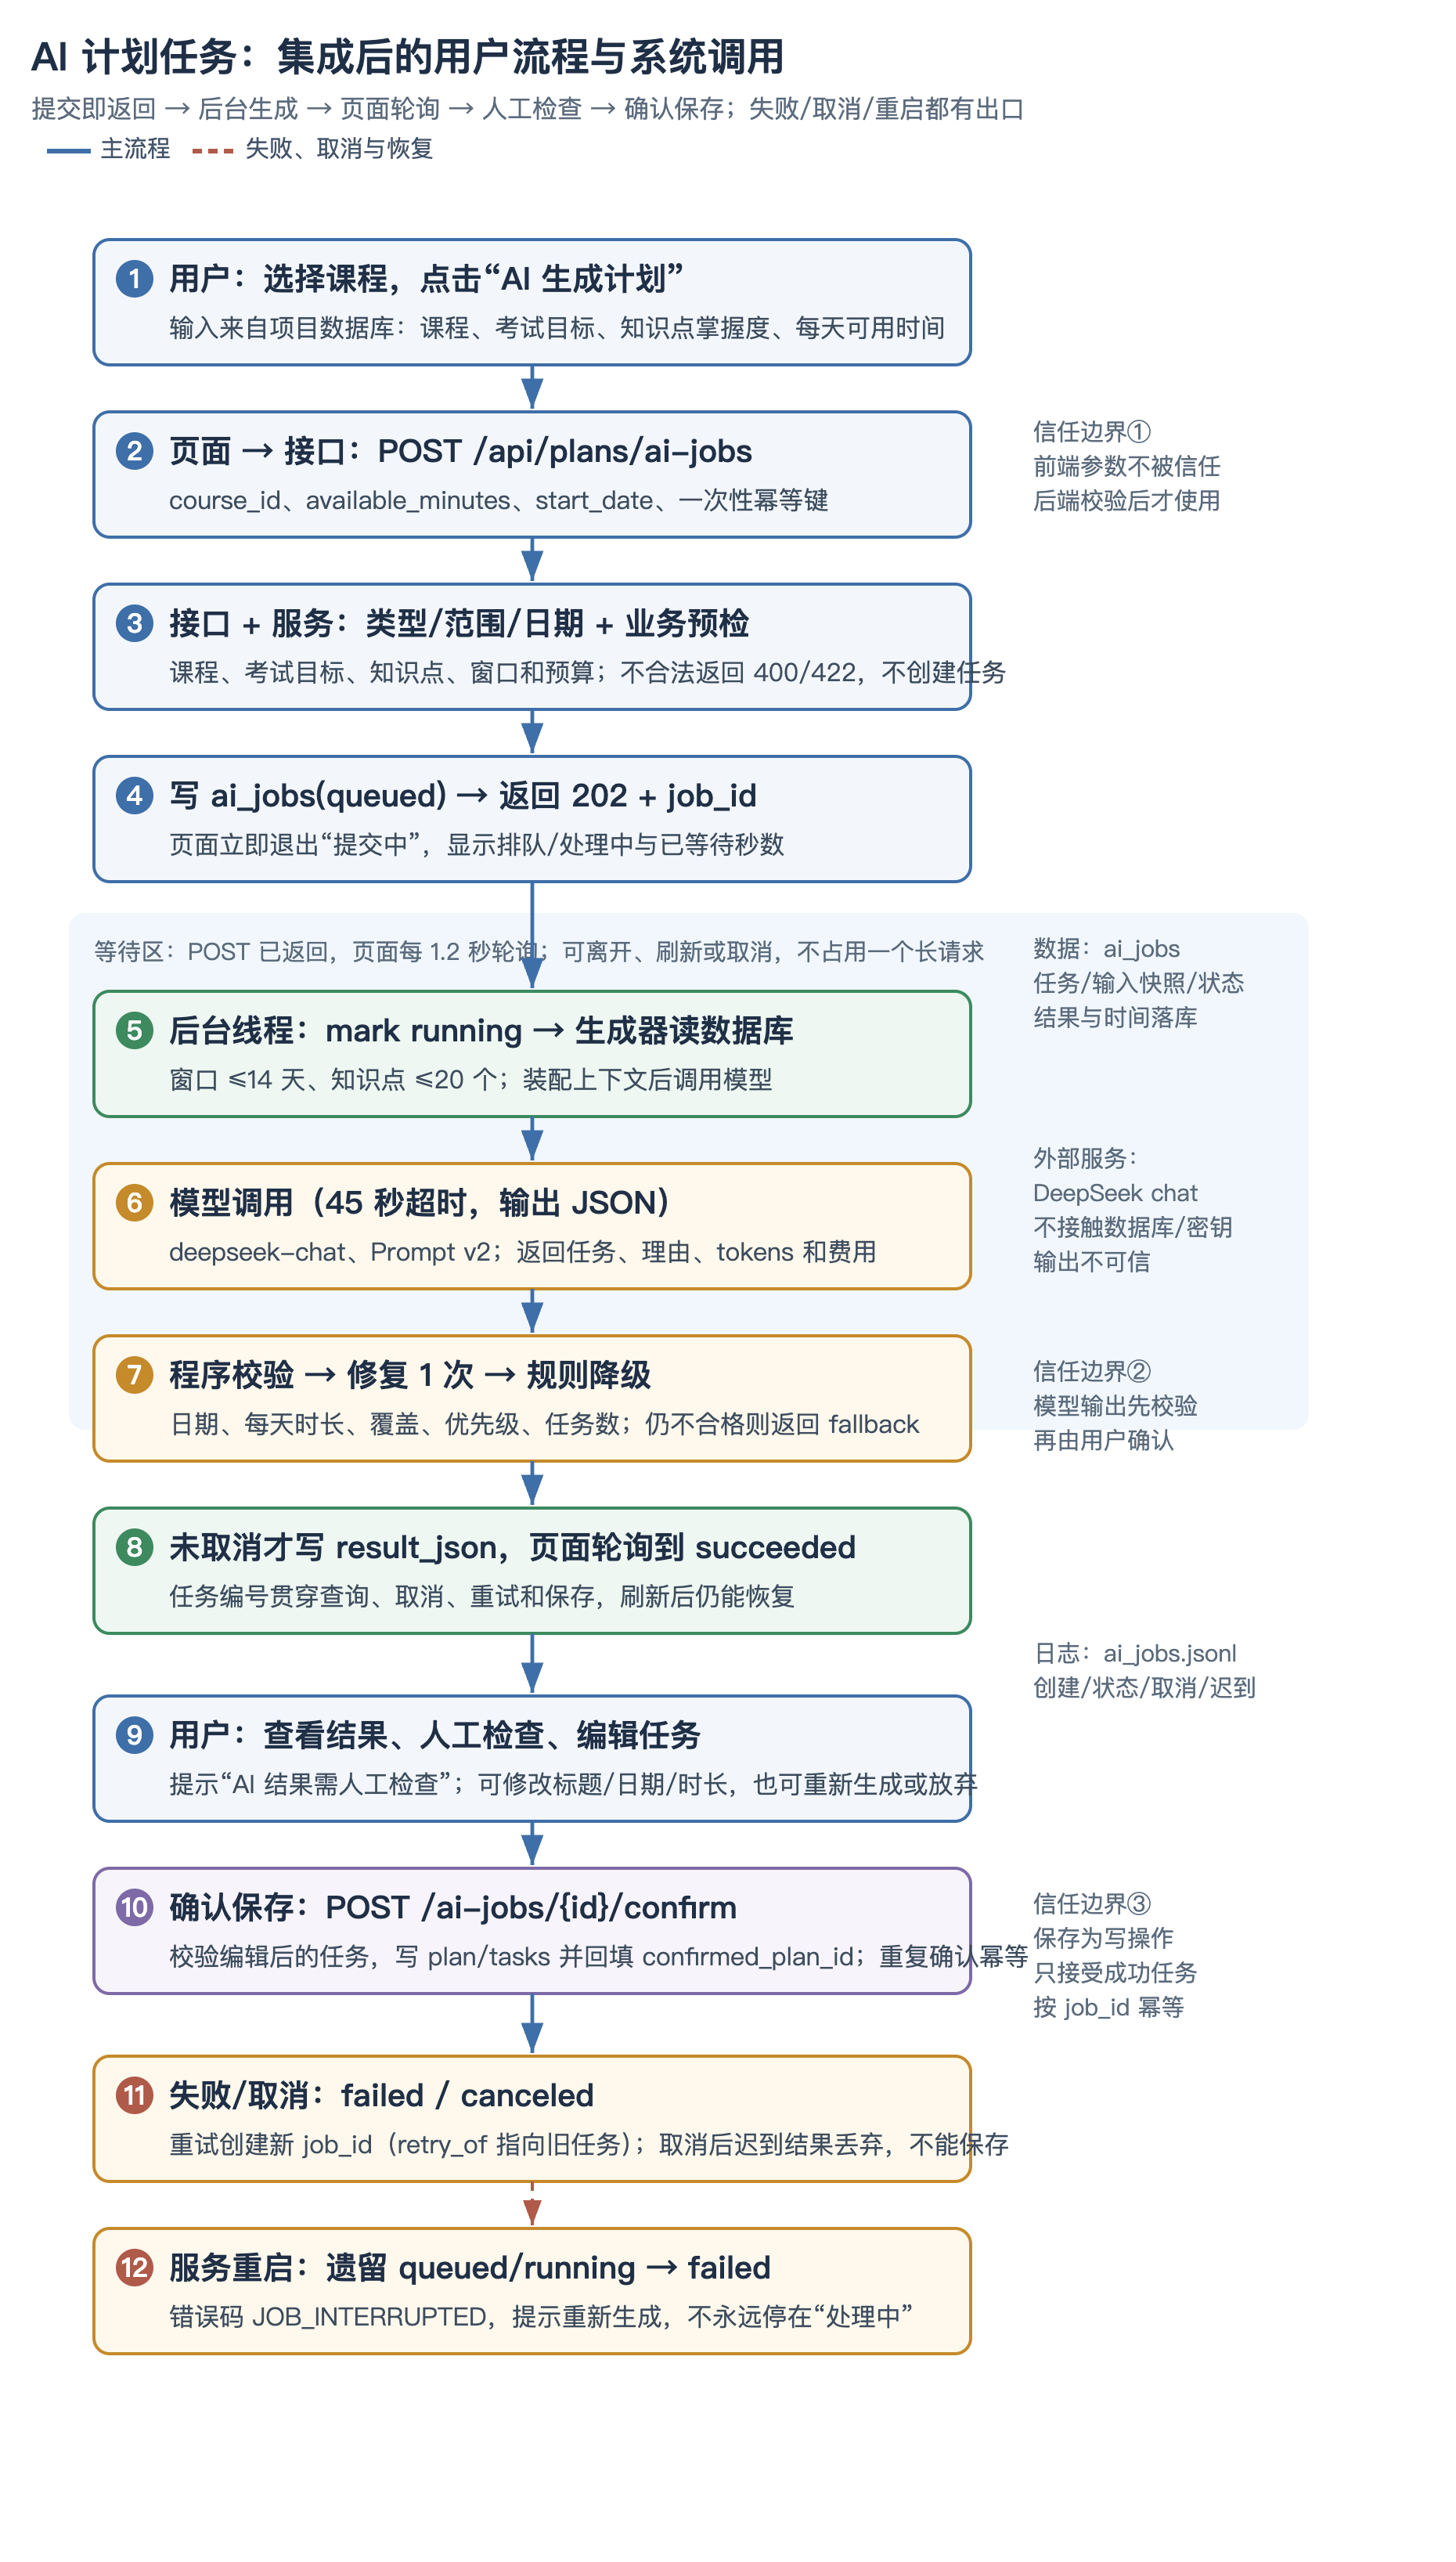
\includegraphics[width=\textwidth]{e8-flow.png}
\caption{AI计划任务的用户流程与系统调用（12步）：等待区、信任边界和失败/取消/恢复出口}
\label{fig:flow}
\end{figure}

各模块的职责和校验位置见表\ref{tab:responsibility}。关键输入校验、状态转换、重复提交判断和保存幂等都在后端完成，页面只负责收集输入和展示状态；模型只输出候选任务，不接触数据库，也没有写入权限。

\begin{table}[H]
\centering
\caption{集成各层的职责与校验位置}
\label{tab:responsibility}
\small
\begin{tabularx}{\textwidth}{L{2.3cm}L{6.0cm}X}
\toprule
模块 & 负责 & 不负责/限制 \\
\midrule
页面（Vue） & 课程选择、按钮提交、轮询、已等待秒数、取消/重试/放弃/编辑、显示错误和结果 & 不判断计划是否可保存；不把未确认结果写库 \\
接口层（FastAPI） & Pydantic 类型/范围/日期格式校验（422）、HTTP 状态码、返回 job\_id & 不解释业务语义，不直接调用模型 \\
任务服务 & 课程/考试目标/知识点预检、任务去重、状态机、取消、重试、保存校验、幂等 & 不生成计划内容，不修改生成器 \\
AI生成器 & 读数据库组装上下文、调用模型、结构化解析、validator、有限修复、规则降级 & 不保存正式计划 \\
数据层（SQLite） & 外键、唯一索引、带前置条件的状态更新、结果与计划写入 & 不做业务判断；单进程部署 \\
模型服务 & 返回候选任务 JSON 与用量 & 输出不可信；不接触数据库和密钥；超时/错误由程序处理 \\
\bottomrule
\end{tabularx}
\end{table}

关于账号和权限：本项目是单用户本地软件，实验4以来就没有账号、登录和角色体系，课程数据属于本机唯一用户。因此本次没有可复用的身份验证和权限检查，任务接口也不做用户归属过滤；能访问本机 8000 端口的人可以看到任务和计划。报告如实说明这一边界，并把它列为后续部署到多用户环境时的改造点：给 \texttt{ai\_jobs} 和课程增加 \texttt{user\_id}、在接口层校验任务归属、再加登录和审计。当前能保证的是“浏览器不直接改状态”：所有状态字段由服务端根据操作转换，客户端提交的 \texttt{status}、\texttt{confirmed\_plan\_id} 等字段一律忽略。

\subsection*{3.2 页面与核心用户流程}

入口沿用实验4的顶部导航“学习计划”（\texttt{\#/plan}），没有新增孤立页面：用户选择课程后看到知识点掌握度，点击“AI 生成计划（后台任务）”，页面立即显示任务编号和“排队中/处理中”，生成完成后任务列表可逐条编辑，最后点“保存为正式计划”。完整流程是：(1)选择课程（已有考试目标和知识点）→(2)提交任务 →(3)等待并轮询 →(4)查看计划与程序校验、人工检查提示 →(5)编辑或重新生成/放弃 →(6)保存为正式计划。图\ref{fig:wait}是提交后的等待态：显示任务编号、状态、已等待秒数和取消入口，没有编造百分比；图\ref{fig:success}是完成态；图\ref{fig:save}是编辑并保存后的状态。

\begin{figure}[htbp]
\centering
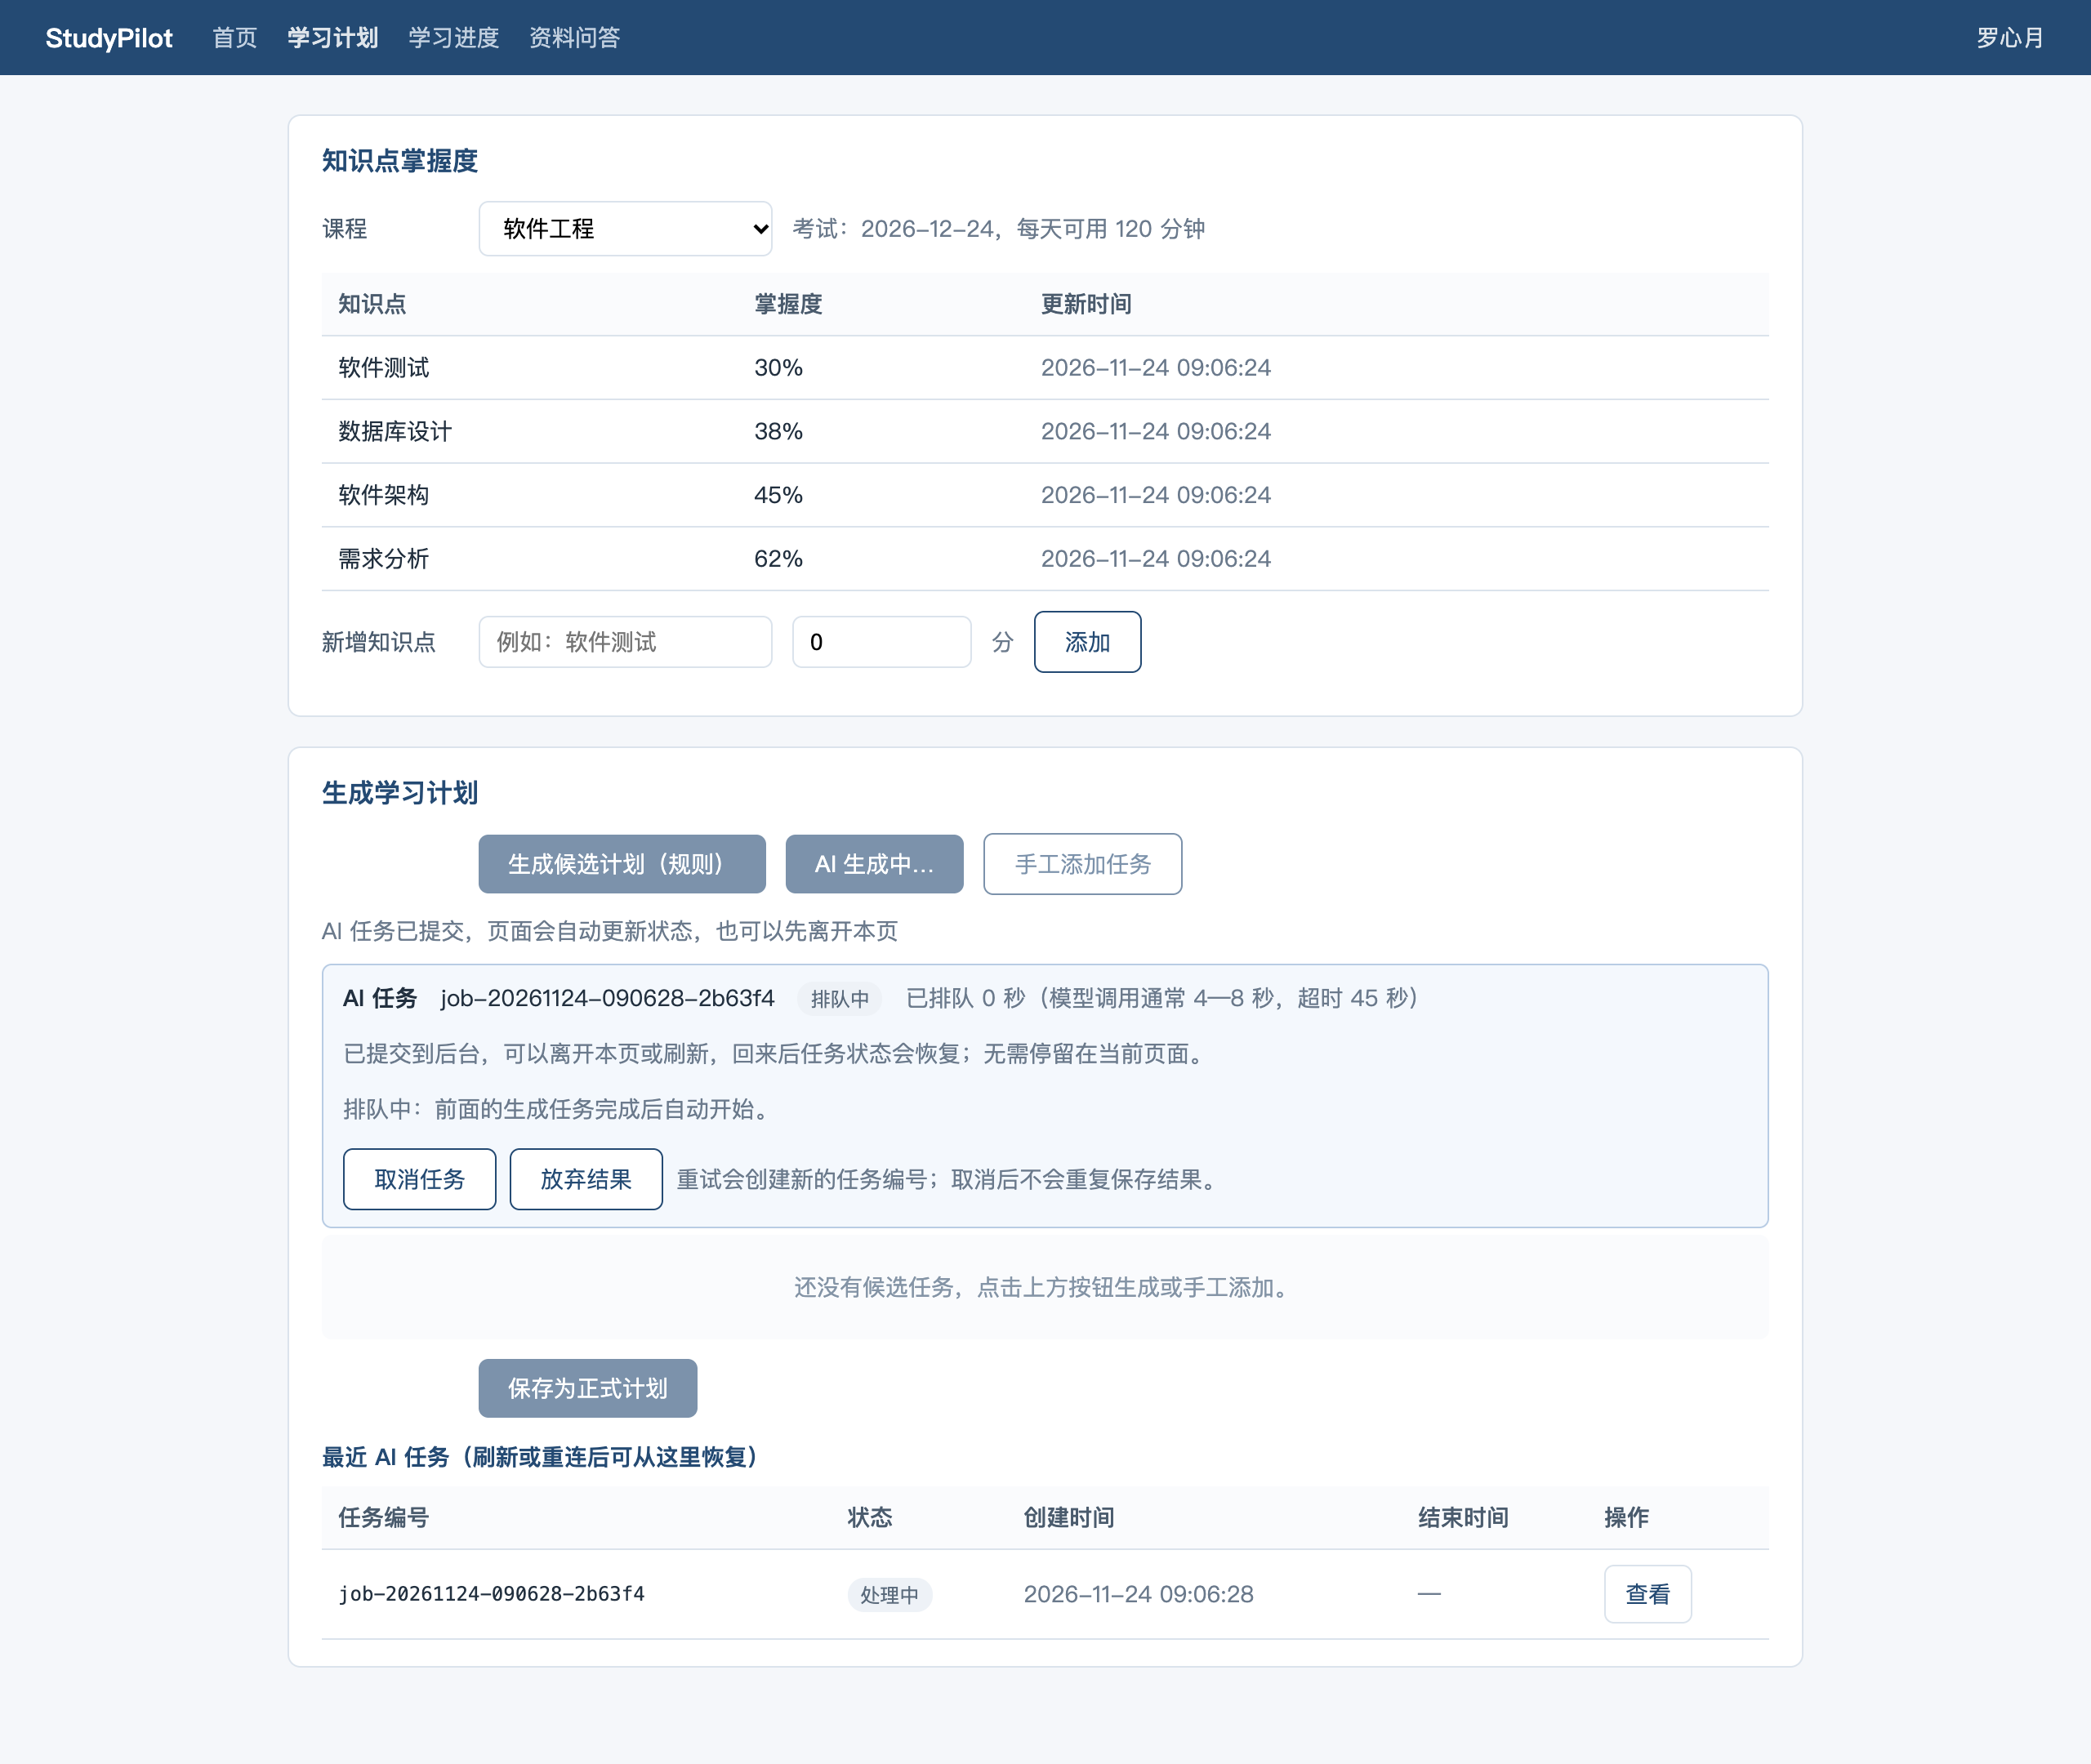
\includegraphics[width=0.92\textwidth]{e8-wait.png}
\caption{等待态：任务编号、排队/处理中状态、已等待秒数和取消入口；明确提示可以离开或刷新}
\label{fig:wait}
\end{figure}

\begin{figure}[htbp]
\centering
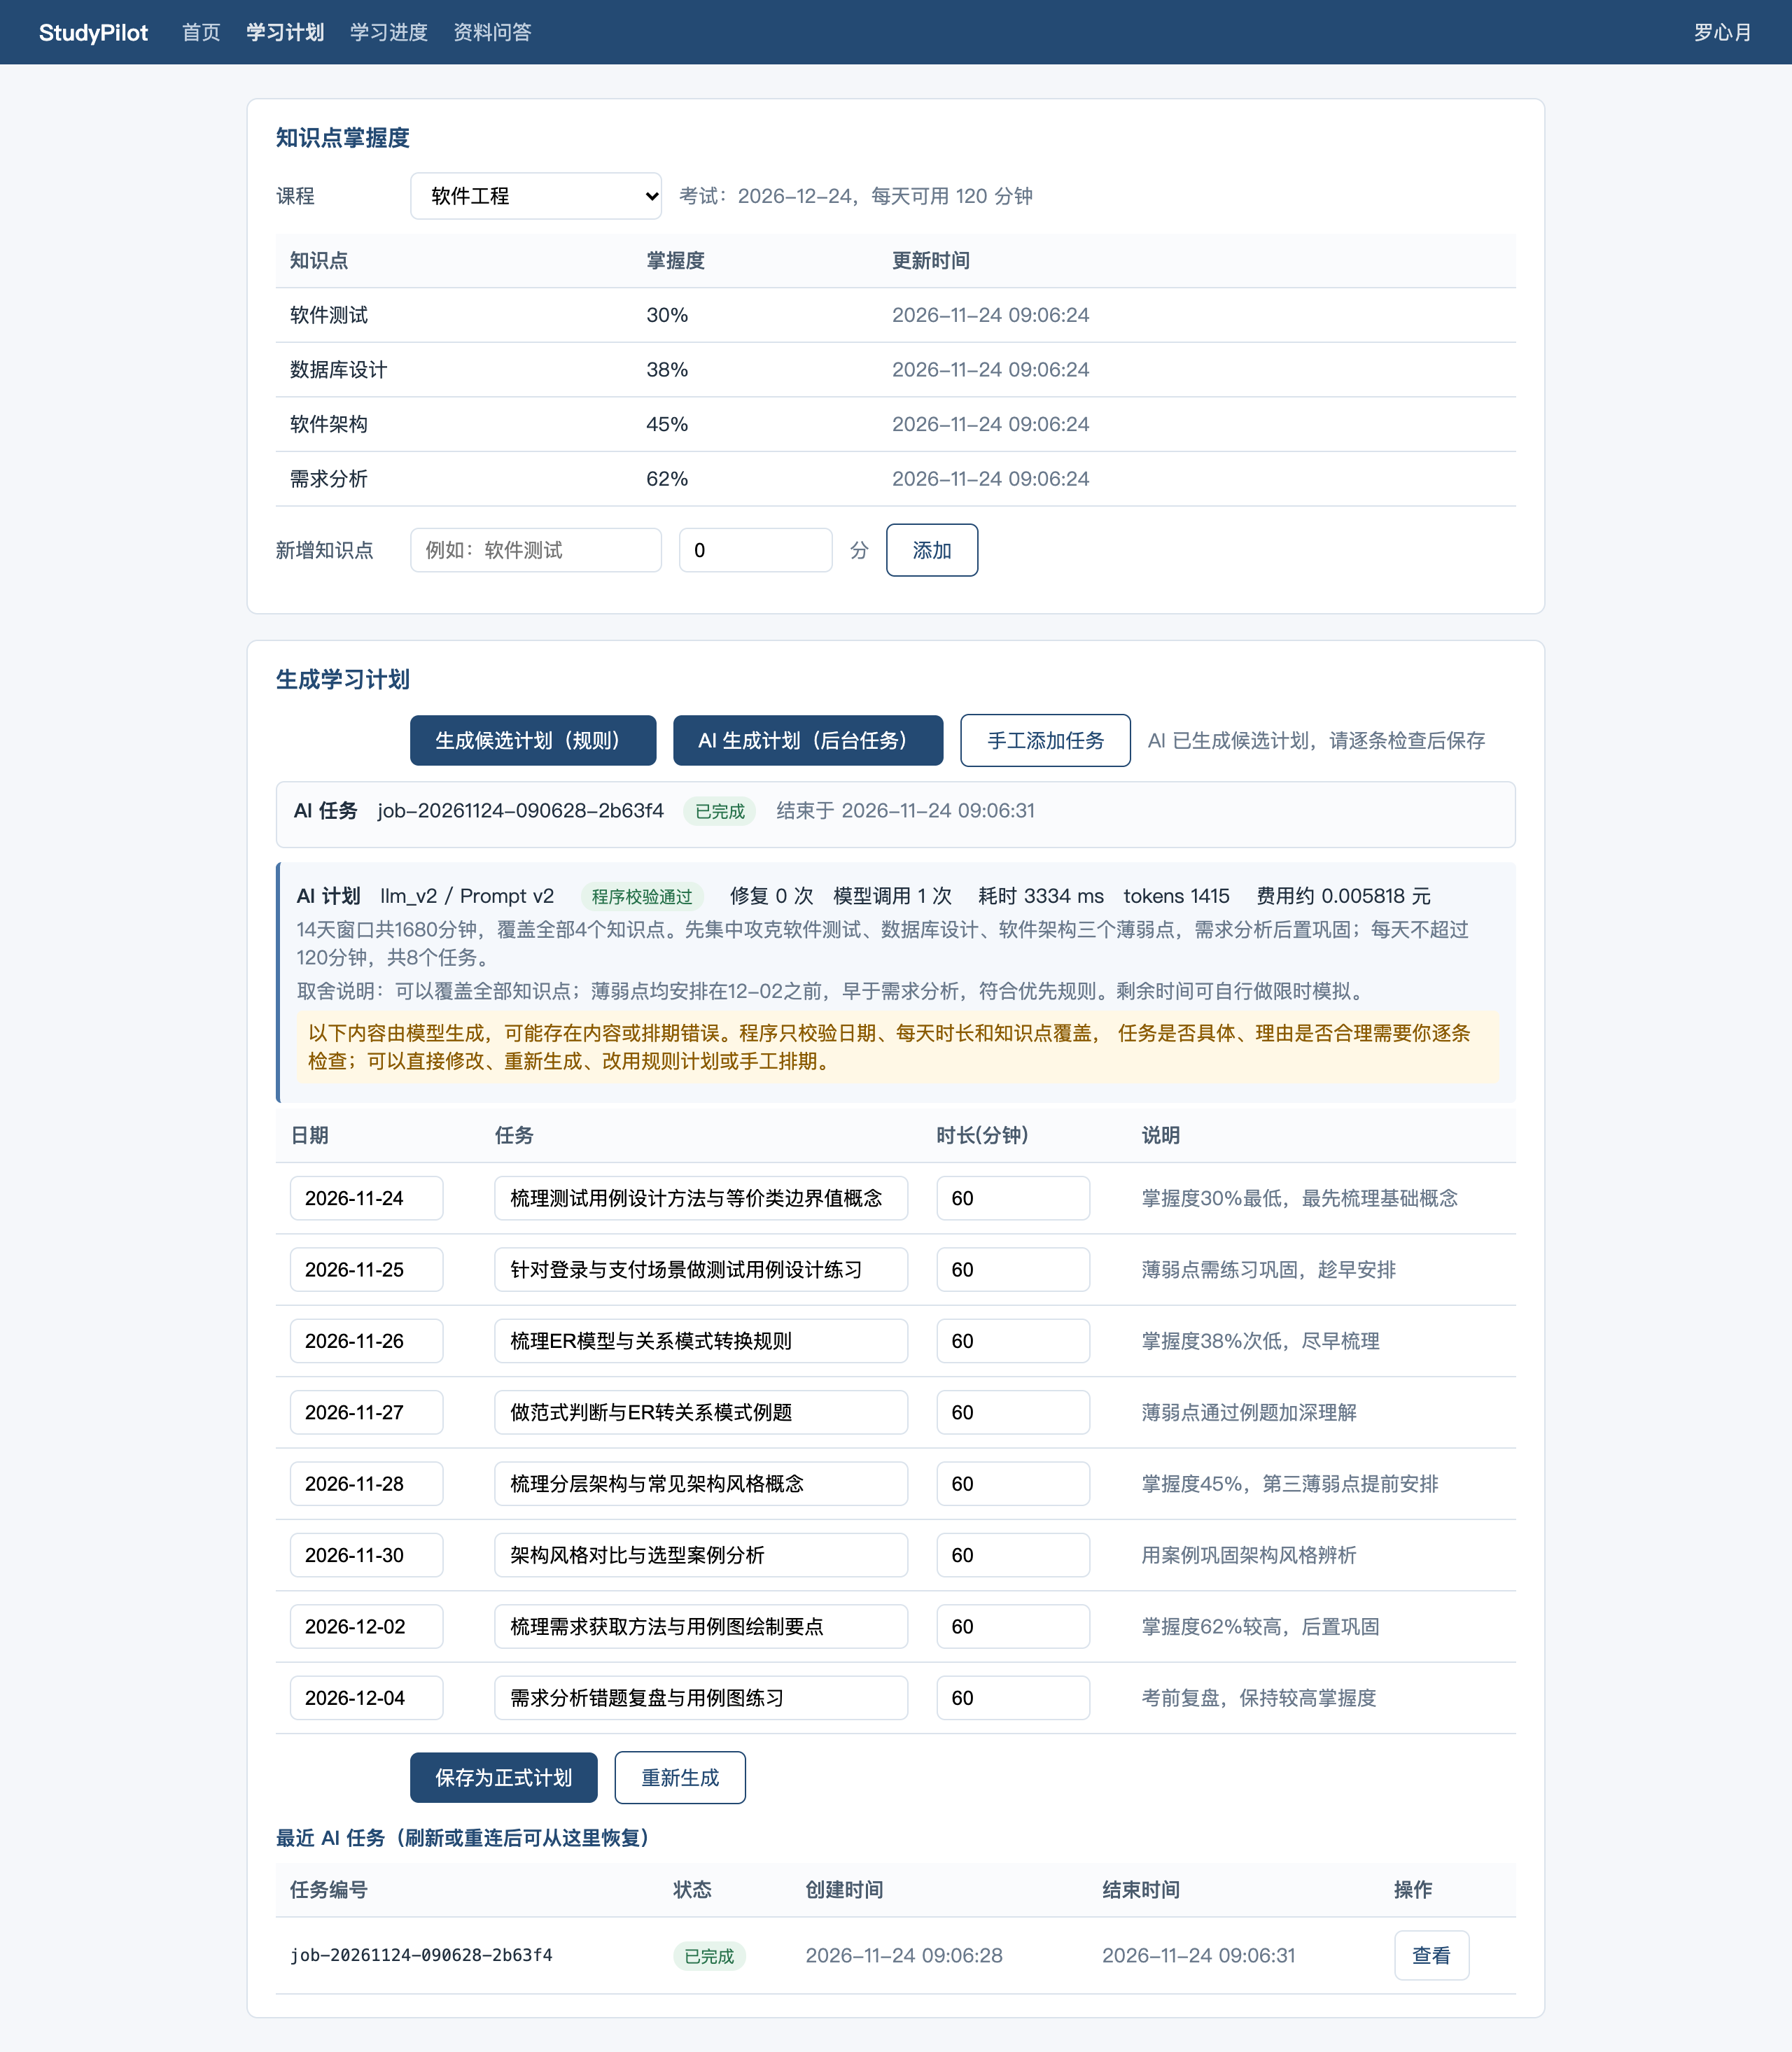
\includegraphics[width=0.92\textwidth]{e8-success.png}
\caption{完成态：计划结果、程序校验、修复次数、耗时、tokens、费用与“需人工检查”提示}
\label{fig:success}
\end{figure}

\begin{figure}[htbp]
\centering
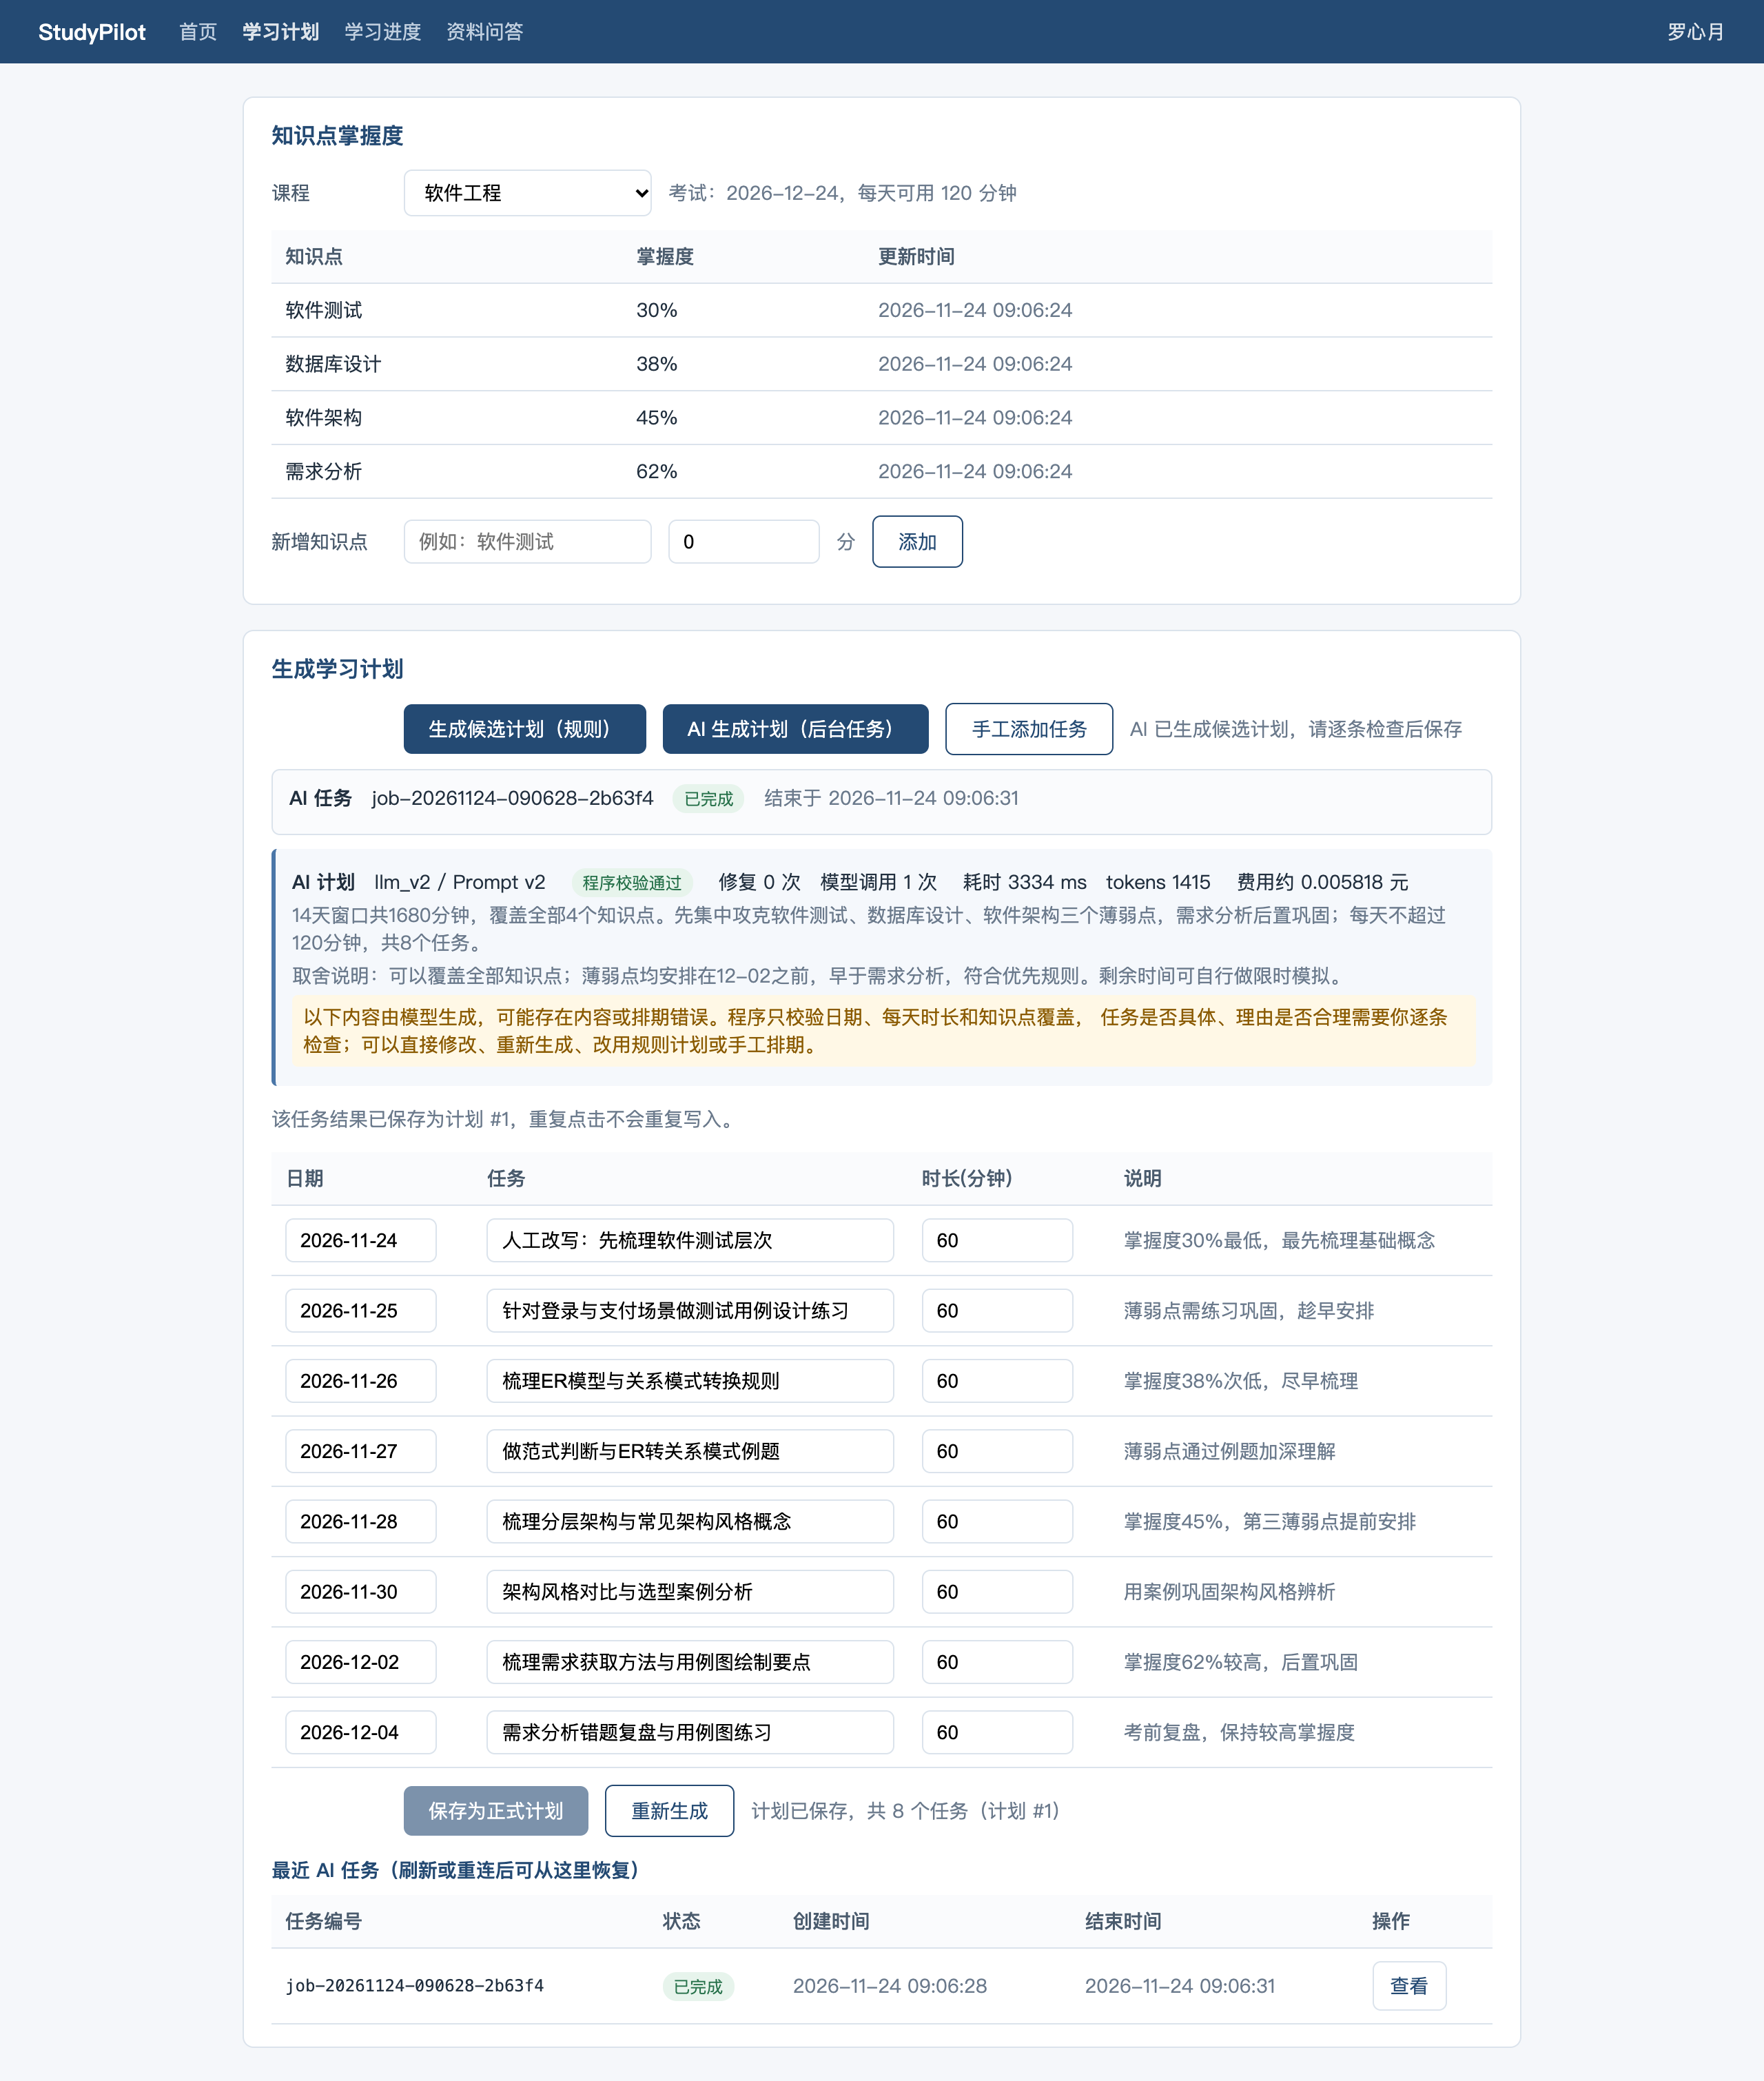
\includegraphics[width=0.88\textwidth]{e8-save.png}
\caption{编辑后保存为正式计划；页面显示计划编号，重复确认由后端幂等处理}
\label{fig:save}
\end{figure}

结果的不确定性用两种方式提示。第一，所有AI结果下方固定显示“以下内容由模型生成，可能存在内容或排期错误；程序只校验日期、每天时长和知识点覆盖，任务是否具体、理由是否合理需要逐条检查”；第二，规则降级时改为“以上为规则模板降级结果（不是模型生成）”，避免把降级结果当成模型结果。用户有四种接力方式：直接修改任务并保存、点“重新生成”再试一次模型、改用“生成候选计划（规则）”、或者“放弃结果”后手工添加任务。任务标题、日期、时长是可编辑输入，知识点编号和程序校验结果只读；保存时提交的是用户编辑后的任务，后端再次校验标题长度、日期格式、时长范围和考试日期，不信任页面限制。

本功能不使用RAG，也没有“来源”需要展示：计划生成的输入全部来自 StudyPilot 自己的 SQLite 数据库（课程、考试目标、知识点掌握度），没有检索外部资料，也没有把教材片段放进上下文。实验5的资料问答页仍单独保留，它的来源展示逻辑没有被这次集成改动。因此2.2中“使用RAG时展示来源”一条对本项目不适用，报告不为此增加假数据。

\subsection*{3.3 状态、会话与数据持久化}

任务状态机见图\ref{fig:state}，转换条件见表\ref{tab:transitions}。状态由服务端写入 SQLite，页面只读；同一门课程同时最多一个 queued/running 任务（部分唯一索引），幂等键相同直接返回已有任务。完成后用户可以保存、重新生成或放弃；失败/取消后可以重试，重试总是创建新任务并把 \texttt{retry\_of} 指向旧任务，旧任务保留在历史里。

\begin{figure}[htbp]
\centering
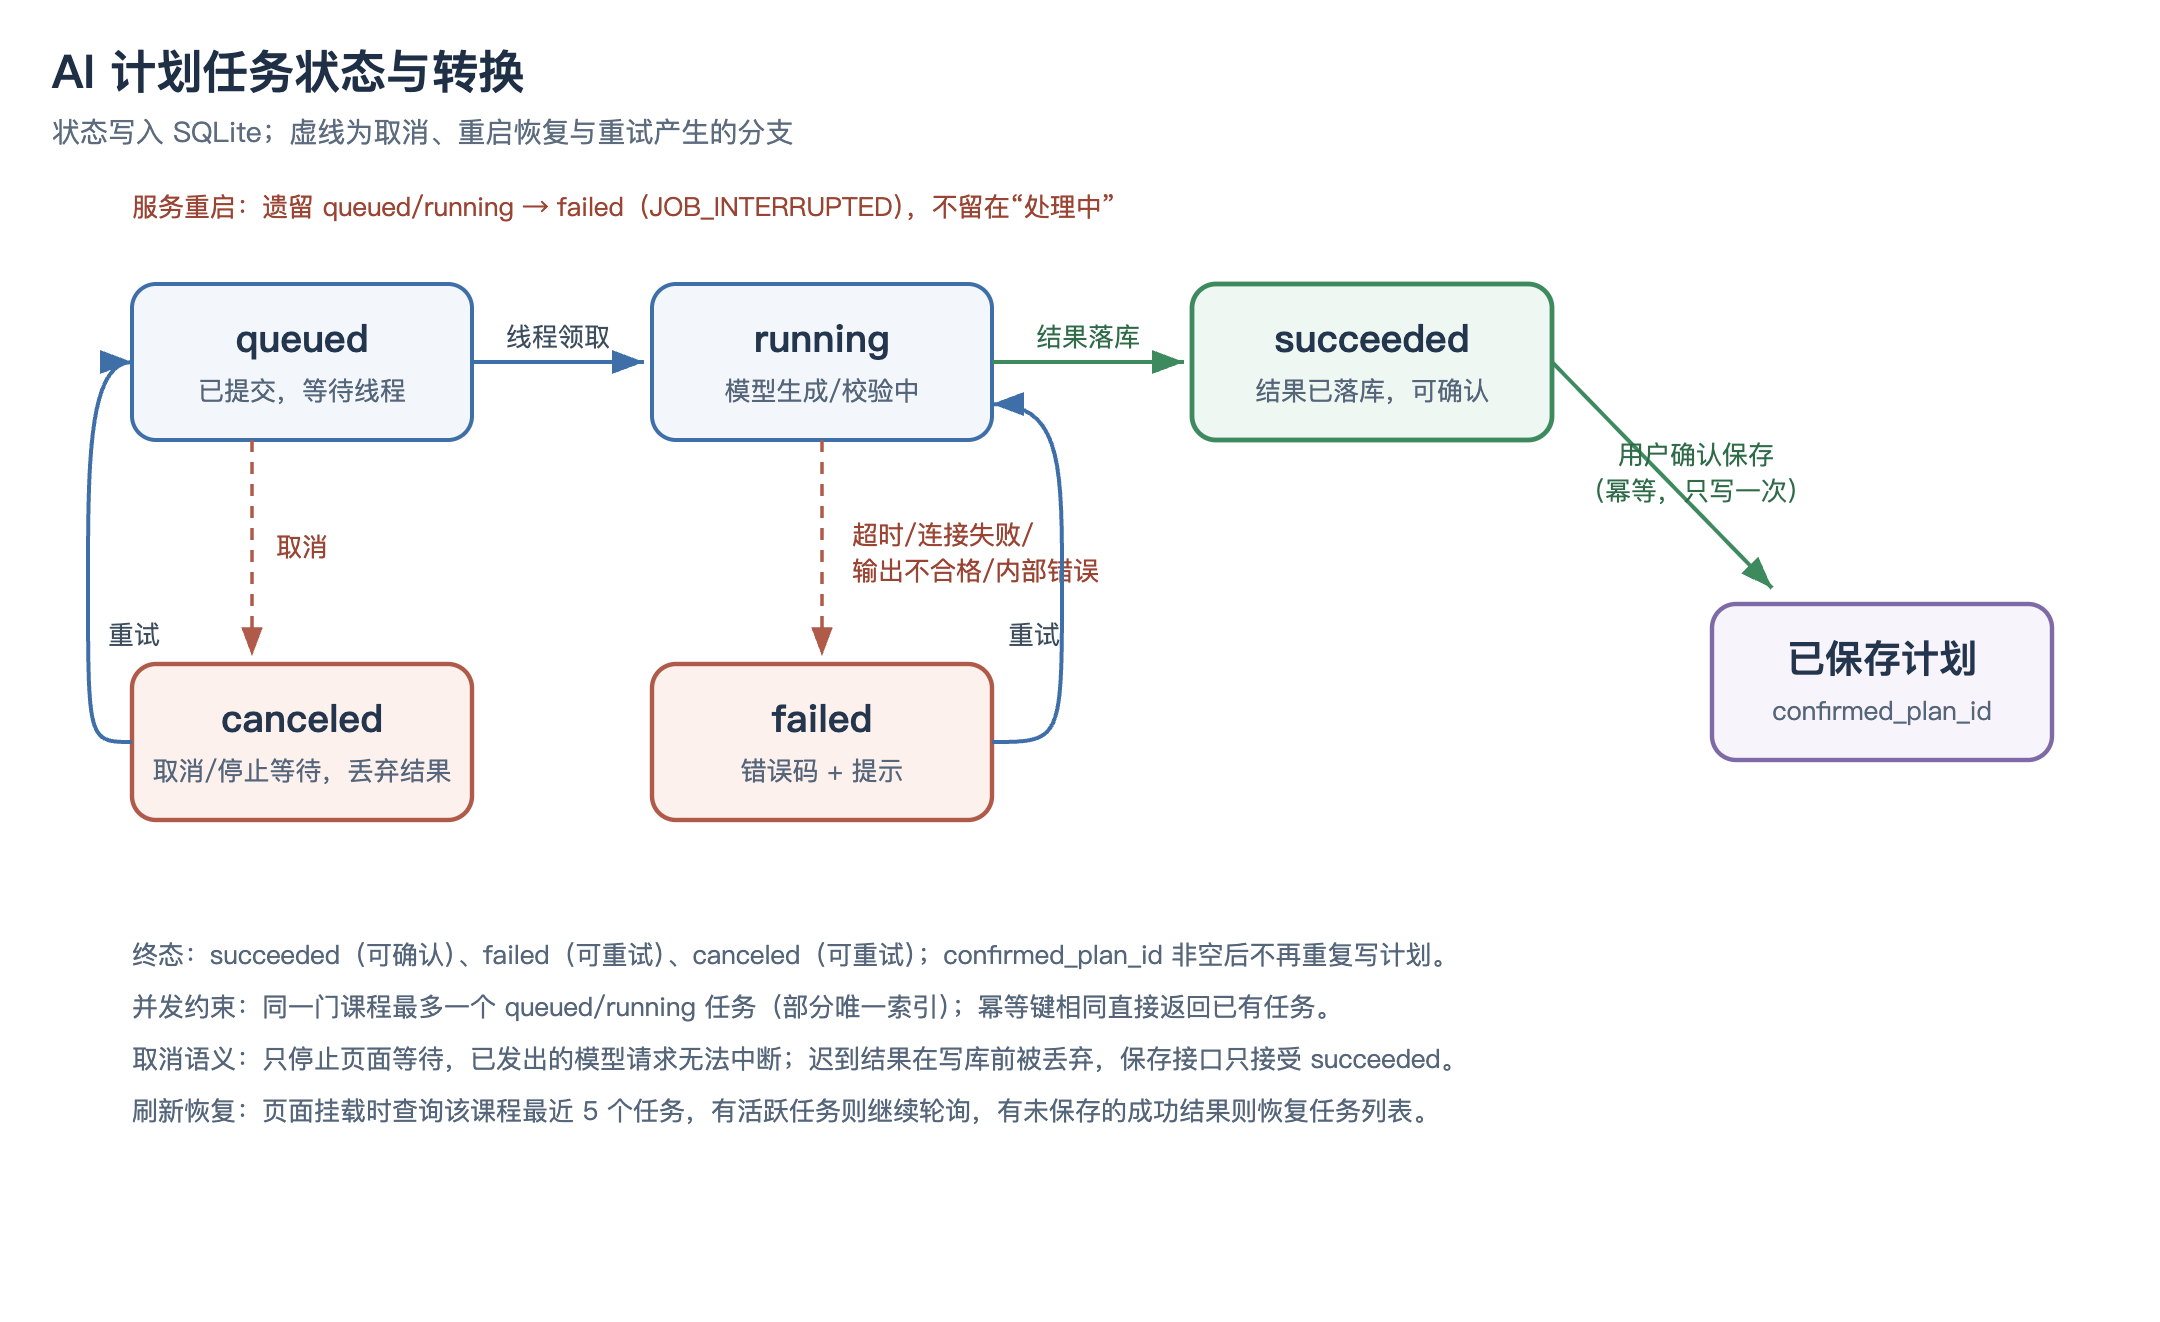
\includegraphics[width=0.98\textwidth]{e8-states.png}
\caption{AI计划任务状态机：正常、失败、取消、重试与启动恢复}
\label{fig:state}
\end{figure}

\begin{table}[H]
\centering
\caption{任务状态转换条件与副作用}
\label{tab:transitions}
\small
\begin{tabularx}{\textwidth}{L{3.0cm}L{2.6cm}L{3.4cm}X}
\toprule
转换 & 触发 & 条件 & 处理与结果 \\
\midrule
queued → running & 后台线程领取 & 状态仍为 queued 且未取消 & \texttt{attempts+1}，写 started\_at \\
queued/running → canceled & 用户点取消 & 状态为 queued 或 running & 立即置 canceled，\texttt{cancel\_requested=1} \\
running → succeeded & 生成器返回 & 未取消且状态仍为 running & 保存 result\_json；模型失败但规则降级也算 succeeded，结果内标 fallback \\
running → failed & 业务异常/未处理异常 & 未取消 & 保存 error\_code/message，任务可重试 \\
failed/canceled → 新任务 & 重试 & 旧任务非成功 & 新 \texttt{job\_id}，\texttt{retry\_of}=旧编号，不继承故障演示参数 \\
succeeded → 已保存 & 用户确认 & 状态 succeeded 且未保存过 & 写 study\_plans/daily\_tasks，回填 confirmed\_plan\_id \\
queued/running → failed & 服务启动恢复 & 上次进程遗留 & JOB\_INTERRUPTED，提示重新生成，不留在“处理中” \\
\bottomrule
\end{tabularx}
\end{table}

表\ref{tab:persistence}说明哪些数据保存、保存多久和如何清理。最终输出（正式计划与每日任务）沿用实验4的表；任务层数据只服务于这次AI生成，没有会话、RAG检索结果或工具调用结果可存，因为本功能不使用它们。

\begin{table}[H]
\centering
\caption{数据保存、用途与清理策略}
\label{tab:persistence}
\small
\begin{tabularx}{\textwidth}{L{3.0cm}L{3.2cm}L{3.8cm}X}
\toprule
数据 & 位置 & 内容 & 保存时间与清理 \\
\midrule
AI任务 & \texttt{ai\_jobs} 表 & 任务编号、课程、状态、输入快照、结果、错误、时间、重试关系、保存关联 & 已结束任务保留 7 天，启动时按 finished\_at 删除更早记录；排队/执行中遗留任务启动时标记中断 \\
正式计划 & \texttt{study\_plans}、\texttt{daily\_tasks} & 保存后的计划与任务（含用户编辑） & 与实验4一致：下次确认同一课程时覆盖旧任务；未做历史版本保留 \\
任务运行日志 & \texttt{backend/logs/ai\_jobs.jsonl} & 创建、开始、完成、取消、失败、迟到结果丢弃 & 追加写入，不自动删除；当前体积很小，后续按需轮转 \\
模型费用/tokens & \texttt{result.meta} 与日志 & 模型、调用次数、tokens、估算费用、耗时 & 随任务记录保留 7 天，页面展示 \\
会话/RAG/工具结果 & 不保存 & 本功能不使用 & 不适用 \\
\bottomrule
\end{tabularx}
\end{table}

\textbf{刷新恢复。}页面挂载时按课程查询最近 5 个任务：若有 queued/running 的任务，直接接入并继续轮询；若有成功但未保存的任务，恢复任务列表和结果；失败/取消只显示状态和重试入口。图\ref{fig:recovery}是任务执行中刷新后的页面，仍在等待同一个任务编号，提示“可以离开本页或刷新，回来后任务状态会恢复”。如果服务进程重启，启动逻辑会把上次未结束的任务标记为 failed（JOB\_INTERRUPTED），页面提示重新生成，而不是永远显示“处理中”。

\begin{figure}[htbp]
\centering
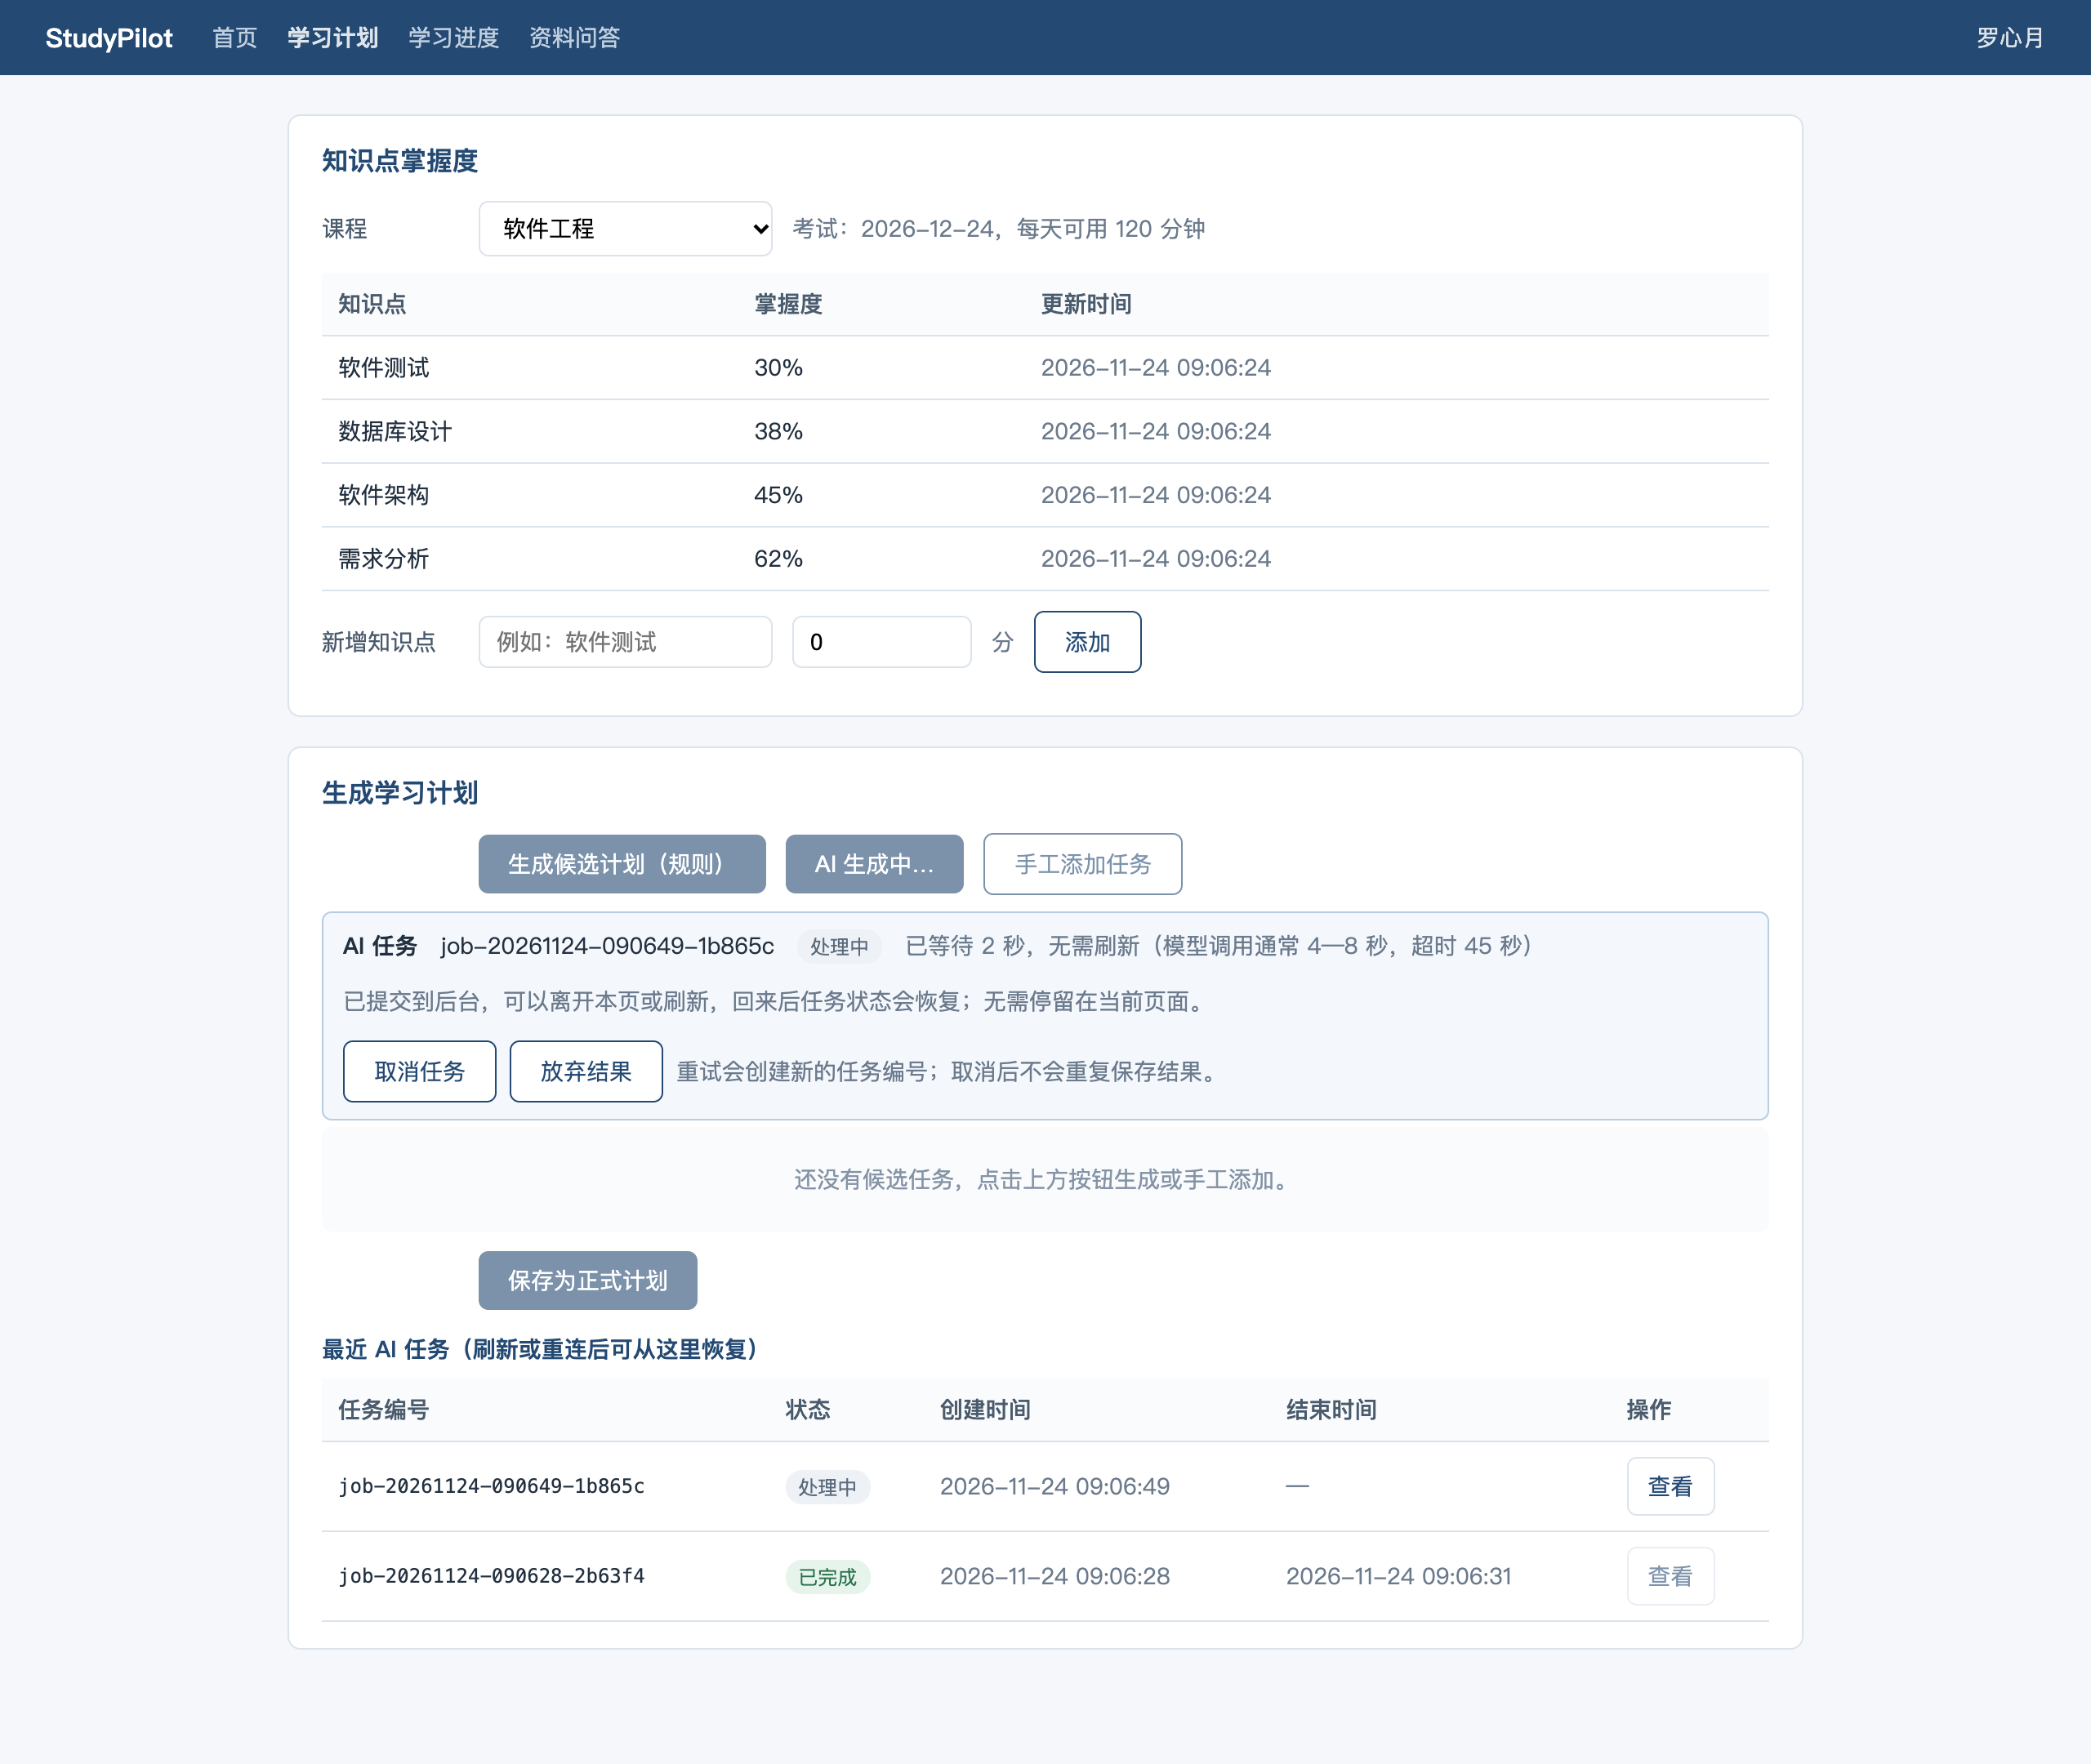
\includegraphics[width=0.92\textwidth]{e8-recovery.png}
\caption{执行中刷新后的恢复：同一任务编号仍在等待，历史任务的“查看”在处理中禁用}
\label{fig:recovery}
\end{figure}

\textbf{取消语义。}取消只停止页面等待并把任务置为 canceled；已经发出的模型 HTTP 请求无法中断，后台线程返回后先检查 \texttt{cancel\_requested}，迟到结果直接丢弃、不写 result\_json，任务也不能再保存。图\ref{fig:cancel}是被取消的任务，2.5 秒后模型结果返回也没有把状态改回成功。若用户取消时任务恰好已经成功，接口返回当前状态而不覆盖成功结果。

\begin{figure}[htbp]
\centering
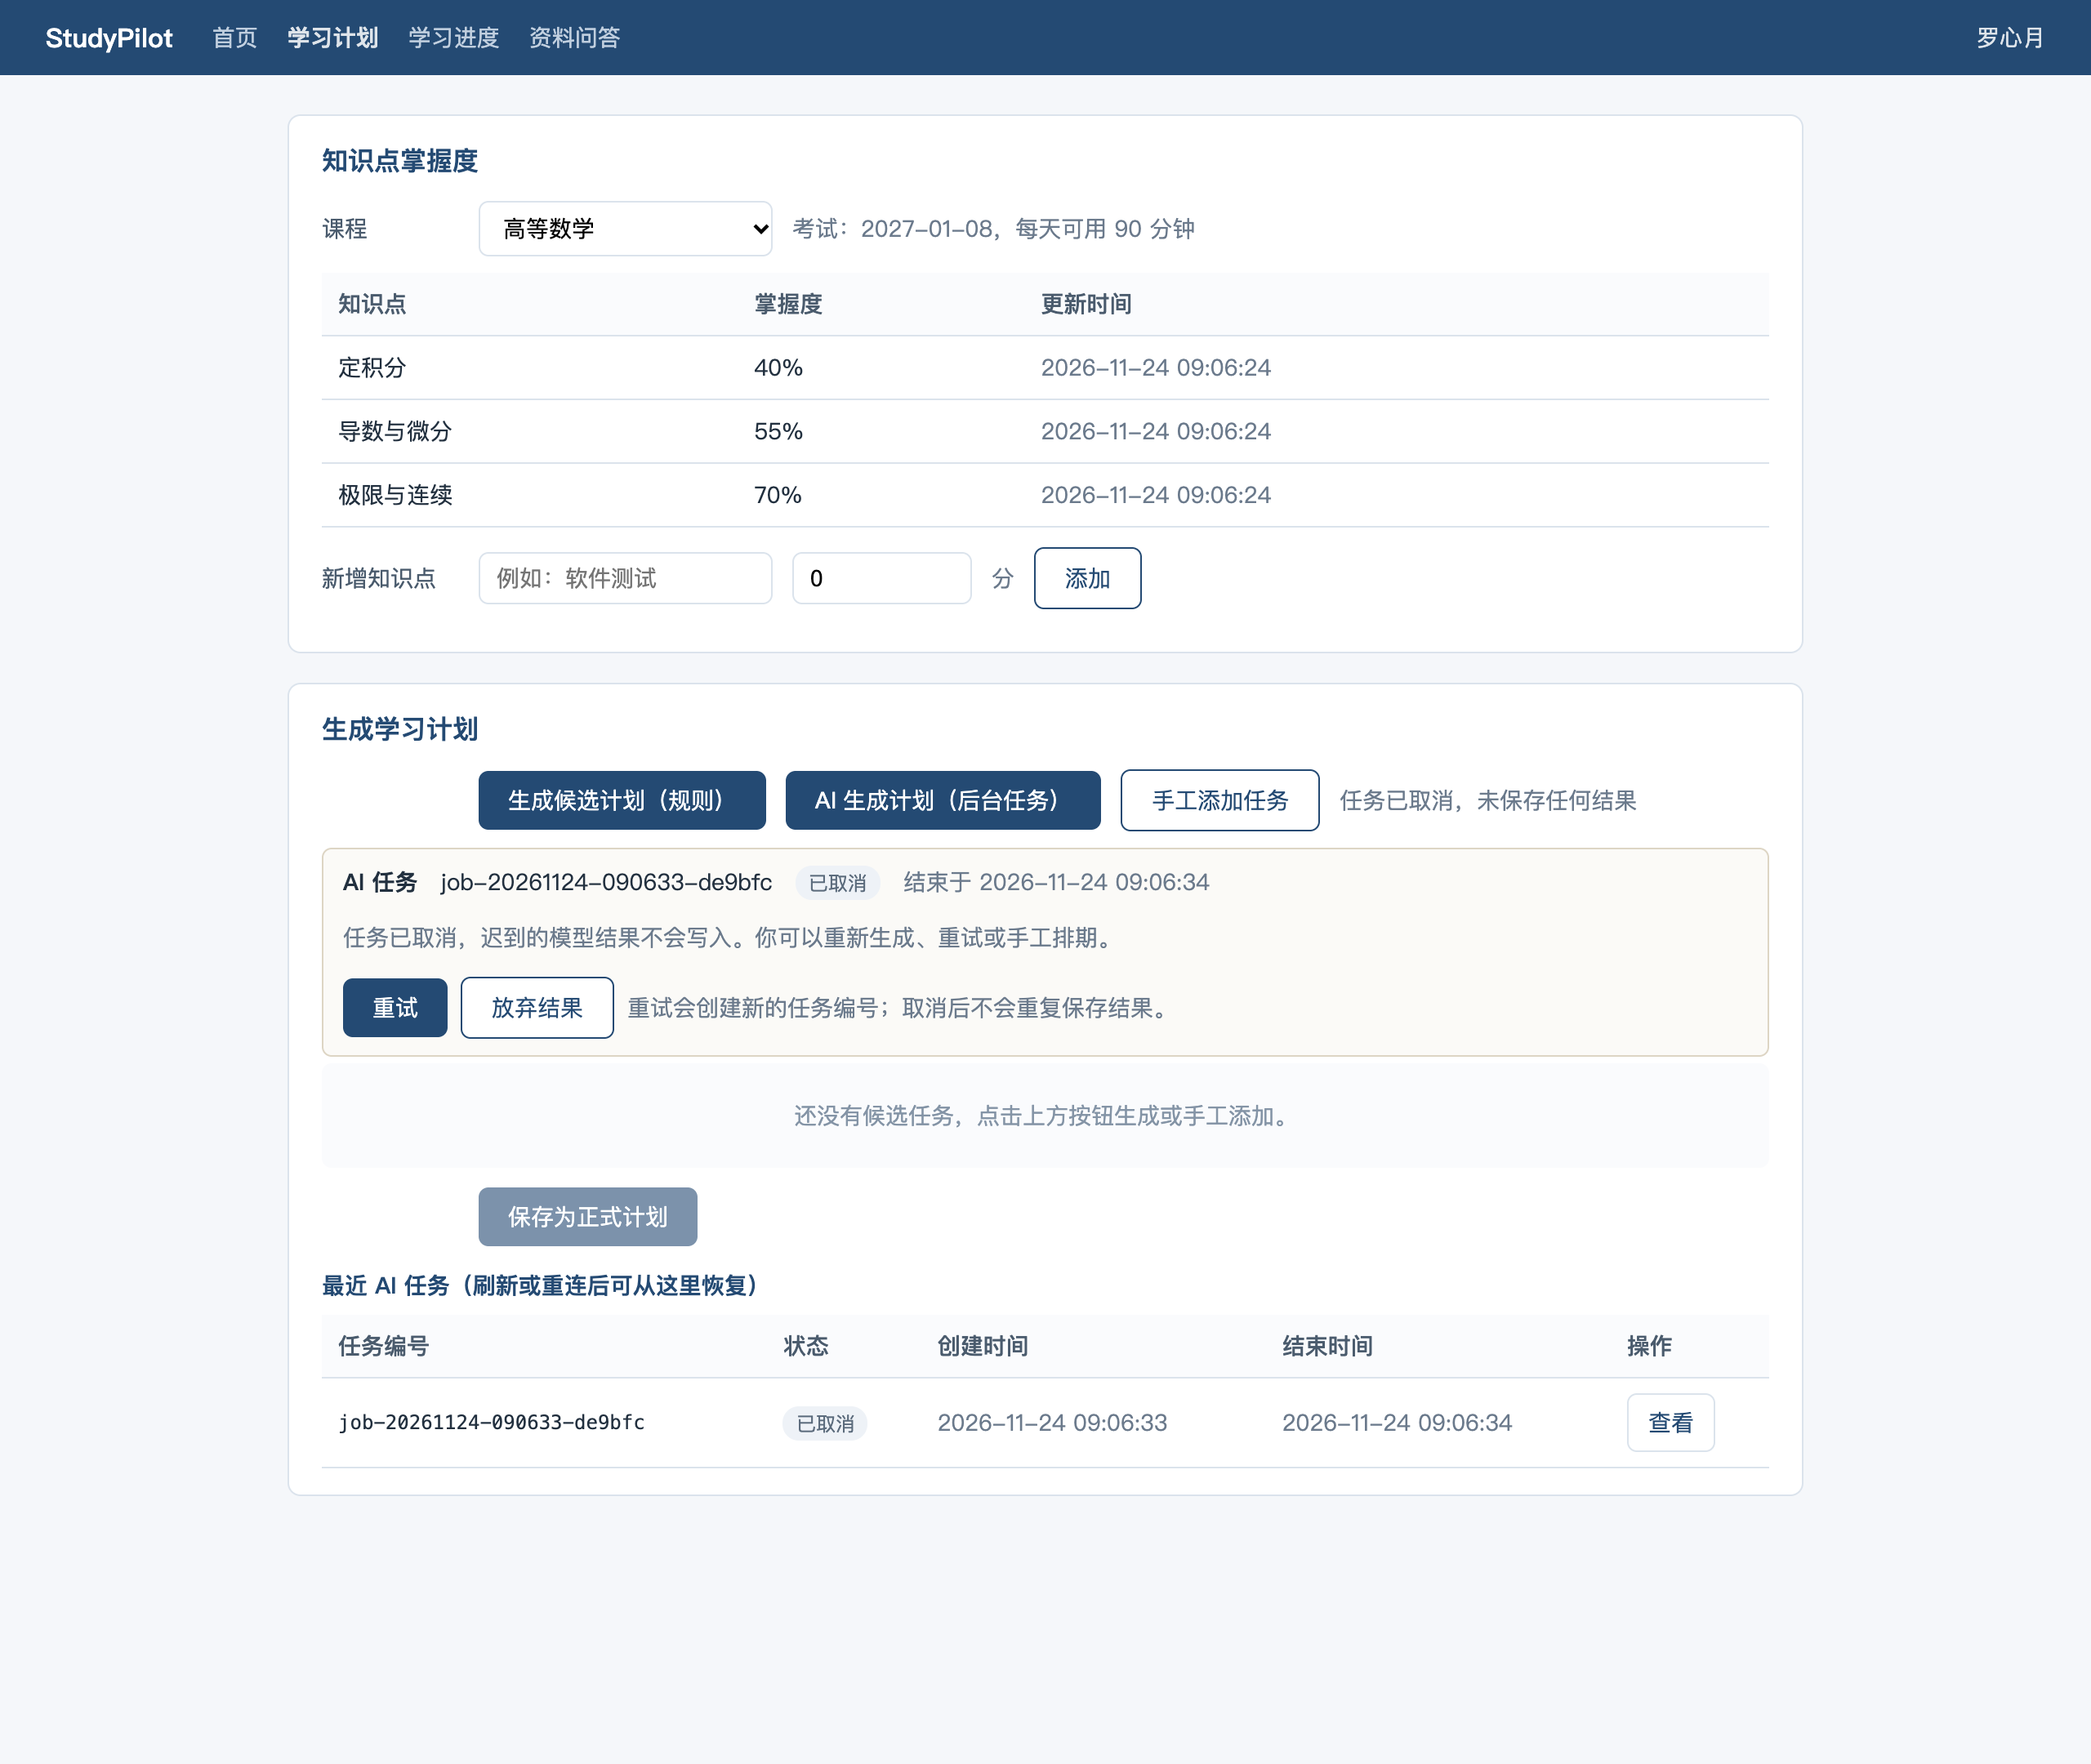
\includegraphics[width=0.92\textwidth]{e8-cancel.png}
\caption{取消态：任务保持已取消、没有AI结果；迟到结果不写入，可重试或改用规则计划}
\label{fig:cancel}
\end{figure}

\textbf{重复提交与交错任务。}同一课程已有排队/执行中任务时，再次提交直接返回原任务并标记 \texttt{deduplicated}，不会重复调用模型；同一幂等键即使旧任务已结束也返回旧任务，避免双击产生两条记录。页面挂载后恢复任务列表，任务编号贯穿状态查询、取消、重试和保存，因此即使交错发起两个任务、返回顺序与提交顺序不同，也不会混用。页面 E2E 场景5同时为软件工程（慢响应）和高等数学提交任务，高等数学先返回、软件工程后返回，两边任务内容分别对应自己的课程；20 个集成测试中的交错用例还验证了保存后两门课程的任务表不混用。

\textbf{会话。}本功能没有多轮对话，不需要会话历史。每次生成是一个独立任务，输入快照保存在 \texttt{request\_json}，结果保存在 \texttt{result\_json}；不同任务之间不共享上下文，也不读取彼此的中间结果。这是本项目的简化选择，报告不虚构“会话恢复”。

\subsection*{3.4 错误提示与降级策略}

错误处理分三层：接口层拦截参数格式问题（422）和明显的业务错误（400/404/409），不创建任务；后台执行层把运行时错误写入 \texttt{job.error}，任务进入 failed；生成器内部对模型超时、连接、限流、鉴权、输出不合格做分类，v2 生成器在无法完成时自动规则降级并返回 fallback 结果。表\ref{tab:errors}列出主要错误、用户提示和可采取的操作。

\begin{table}[H]
\centering
\caption{主要错误、状态与用户可采取的操作}
\label{tab:errors}
\footnotesize
\begin{tabularx}{\textwidth}{L{4.2cm}L{3.3cm}L{3.6cm}X}
\toprule
错误码 & 触发场景 & 用户看到的状态与提示 & 可采取操作 \\
\midrule
INVALID\_PARAMETER（422） & 参数类型、范围或日期格式不合法 & 请求参数不完整或格式错误 & 修改输入后重新提交；不创建任务 \\
COURSE\_NOT\_FOUND\newline GOAL\_NOT\_FOUND\newline EMPTY\_KNOWLEDGE\_POINTS & 课程、考试目标或知识点缺失 & 明确提示先补哪一项 & 去设置考试目标或添加知识点；不创建任务 \\
TOO\_MANY\_POINTS\newline NO\_AVAILABLE\_DAY\newline INVALID\_AVAILABLE\_MINUTES & 超出原型能力或窗口 & 说明上限和当前值 & 拆分知识点、调整日期或可用时间；不创建任务 \\
JOB\_NOT\_SUCCEEDED（409） & 未成功任务点保存 & 任务当前状态，只有成功任务能保存 & 等待完成或重试；不会写计划 \\
JOB\_NOT\_RETRYABLE（409） & 对成功任务点重试 & 只有失败或已取消任务可重试 & 用“重新生成”而不是重试 \\
INVALID\_TASK\_*\newline TASK\_DATE\_AFTER\_EXAM & 编辑后的任务不合法 & 指出第几条、哪个字段不合法 & 修改任务；任务仍未保存 \\
LLM\_TIMEOUT\newline LLM\_CONNECTION\_ERROR & 模型超时或连接失败 & 失败原因 + “可重试或改用规则计划” & 重试（新任务）、规则生成、手工排期 \\
LLM\_NOT\_CONFIGURED\newline LLM\_AUTH\_FAILED\newline LLM\_RATE\_LIMITED & 未配置密钥、鉴权失败、限流 & 生成器降级，页面显示降级原因与规则结果 & 仍可编辑保存规则计划；稍后重新生成 \\
输出两次不合格 & validator 未通过且修复失败 & 任务成功但 result.status=fallback & 查看降级原因，手工调整后保存 \\
JOB\_INTERRUPTED & 服务重启时任务未结束 & 提示任务中断，请重新生成 & 重新生成或重试 \\
DATABASE\_UNAVAILABLE & 数据库暂时不可用 & 提示稍后重试，已保存计划不受影响 & 稍后重试；轮询失败时页面保留状态并继续重试 \\
\bottomrule
\end{tabularx}
\end{table}

图\ref{fig:failed}是模拟模型超时后的失败页：显示失败原因、错误码、可采取的操作，以及“重试”“放弃结果”按钮；图\ref{fig:retry}是点重试后新任务成功的结果（这次重试实际触发了两次模型调用与一次修复，耗时约 7.5 秒）。重试会创建新任务编号，旧失败任务保留在历史中，因此不会覆盖证据，也不会重复保存计划。

\begin{figure}[htbp]
\centering
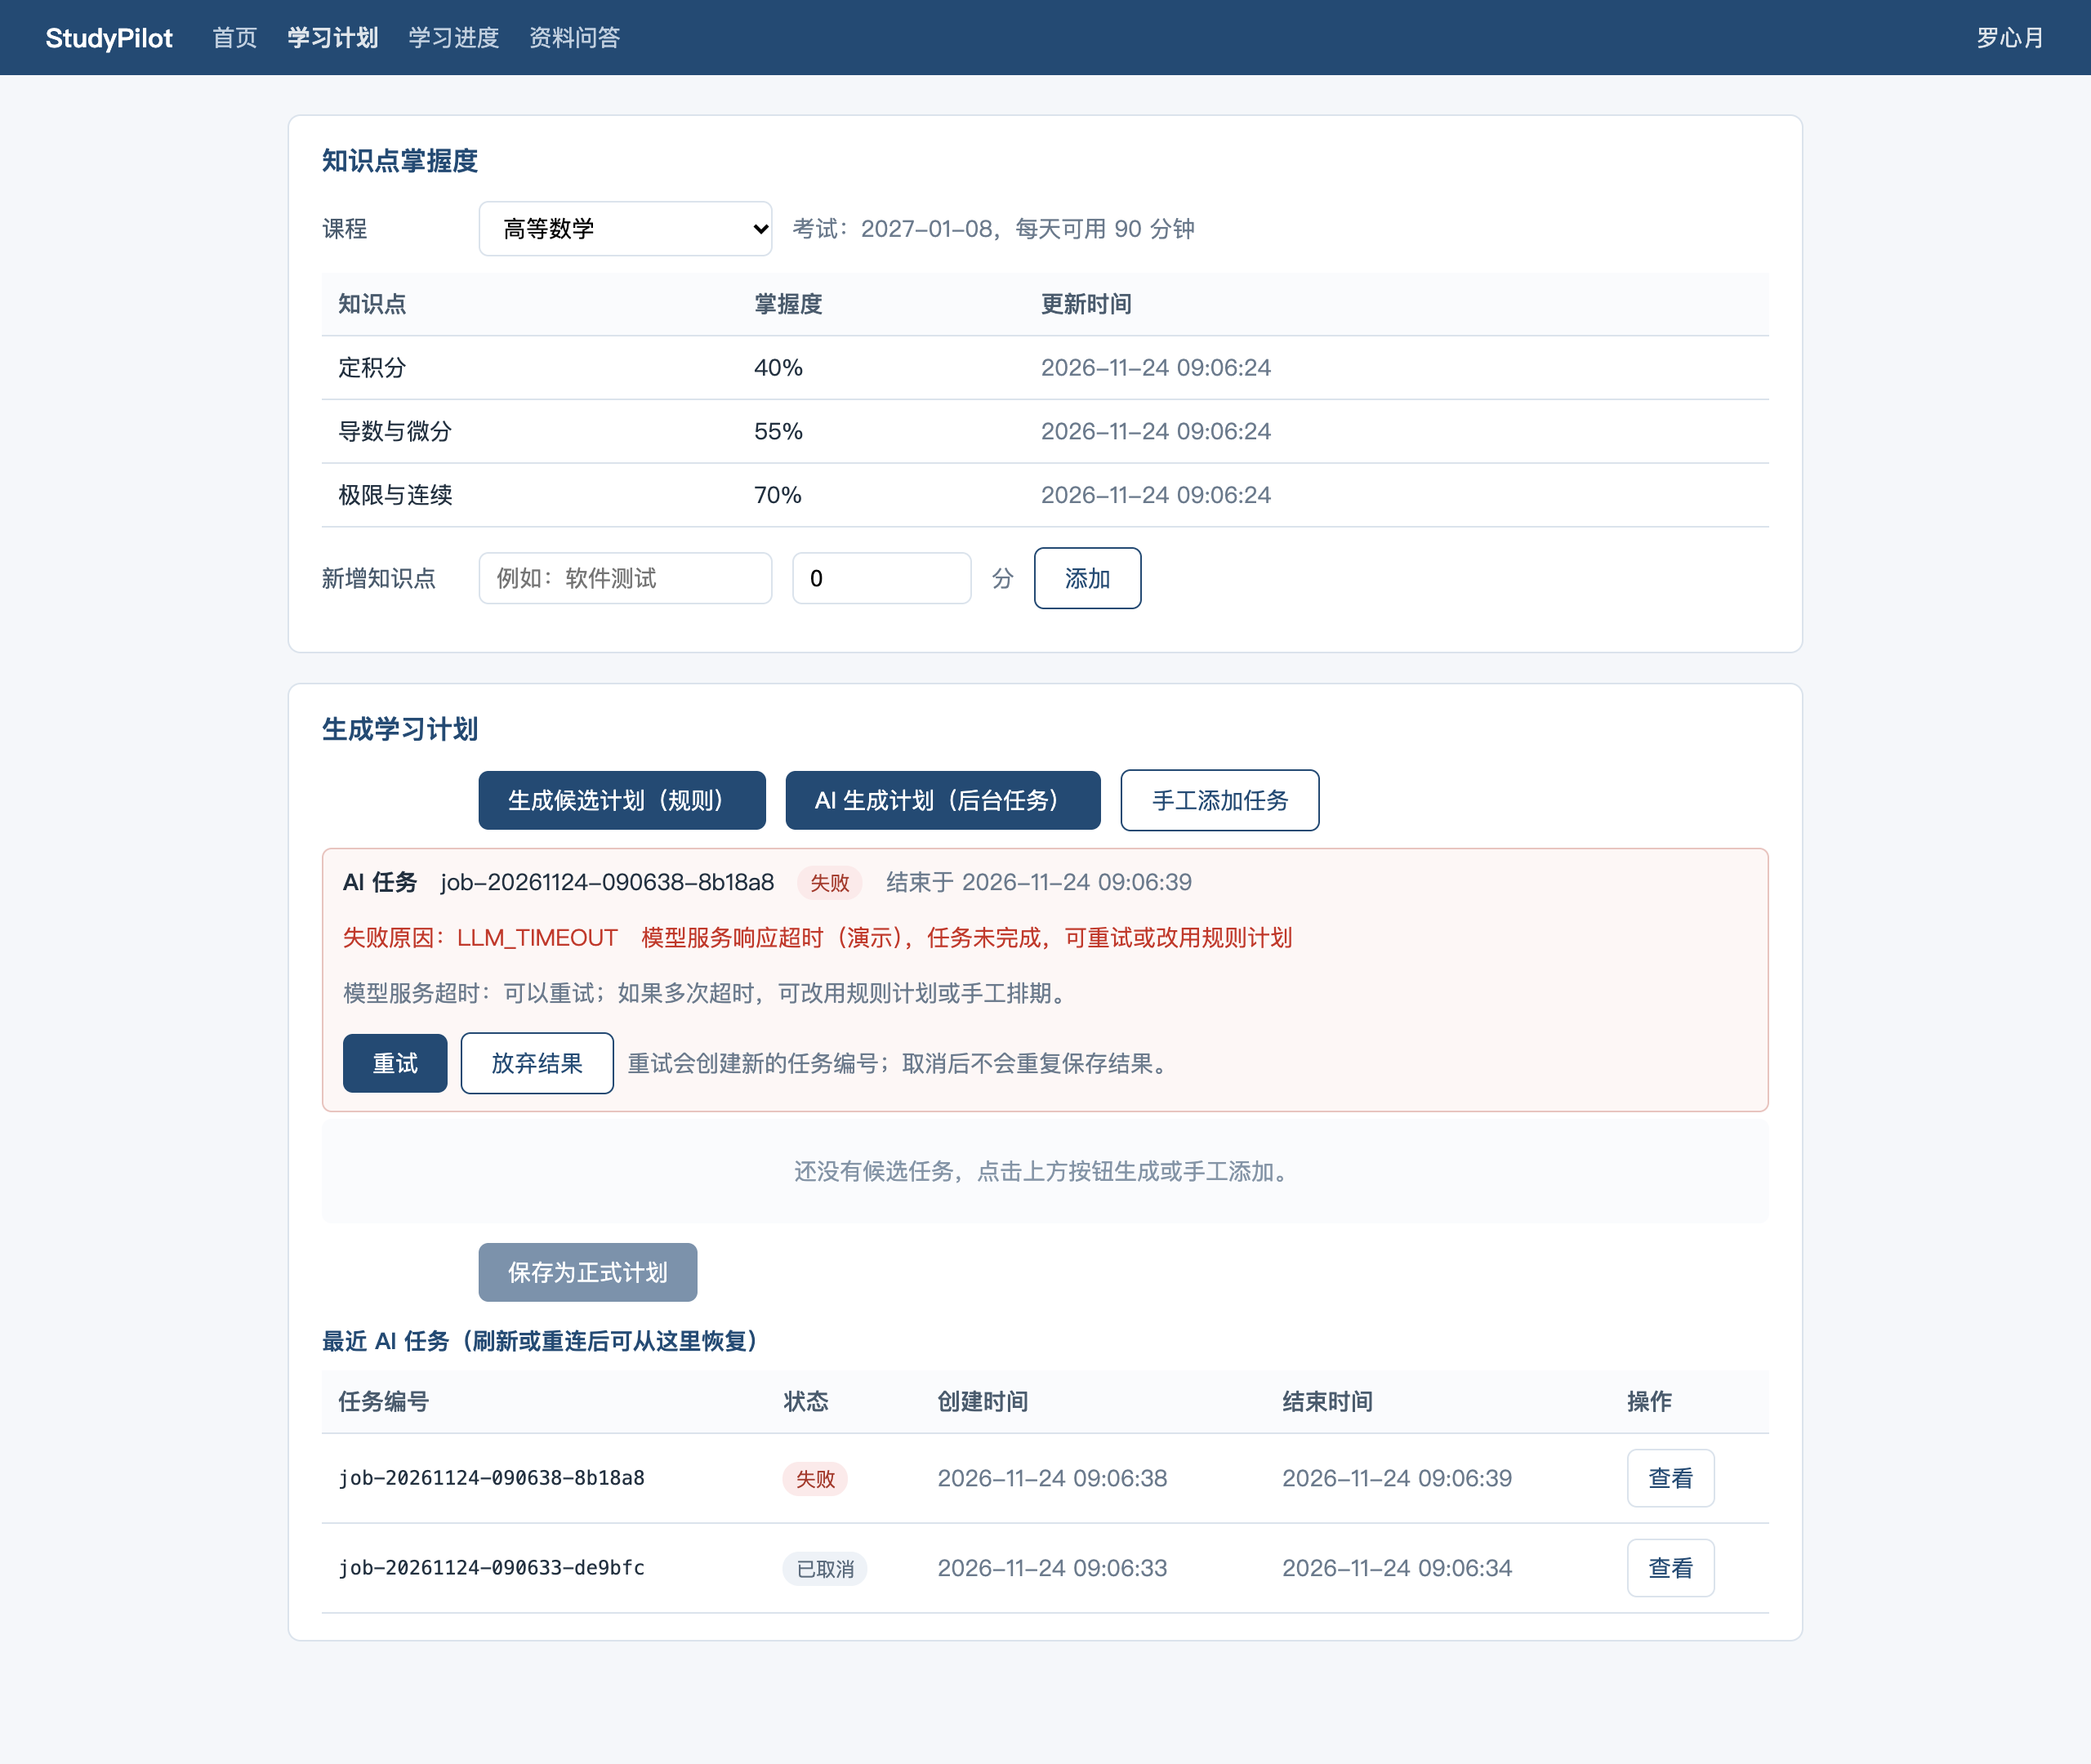
\includegraphics[width=0.92\textwidth]{e8-failed.png}
\caption{失败态：错误码、原因和“重试/规则生成/手工排期”提示}
\label{fig:failed}
\end{figure}

\begin{figure}[htbp]
\centering
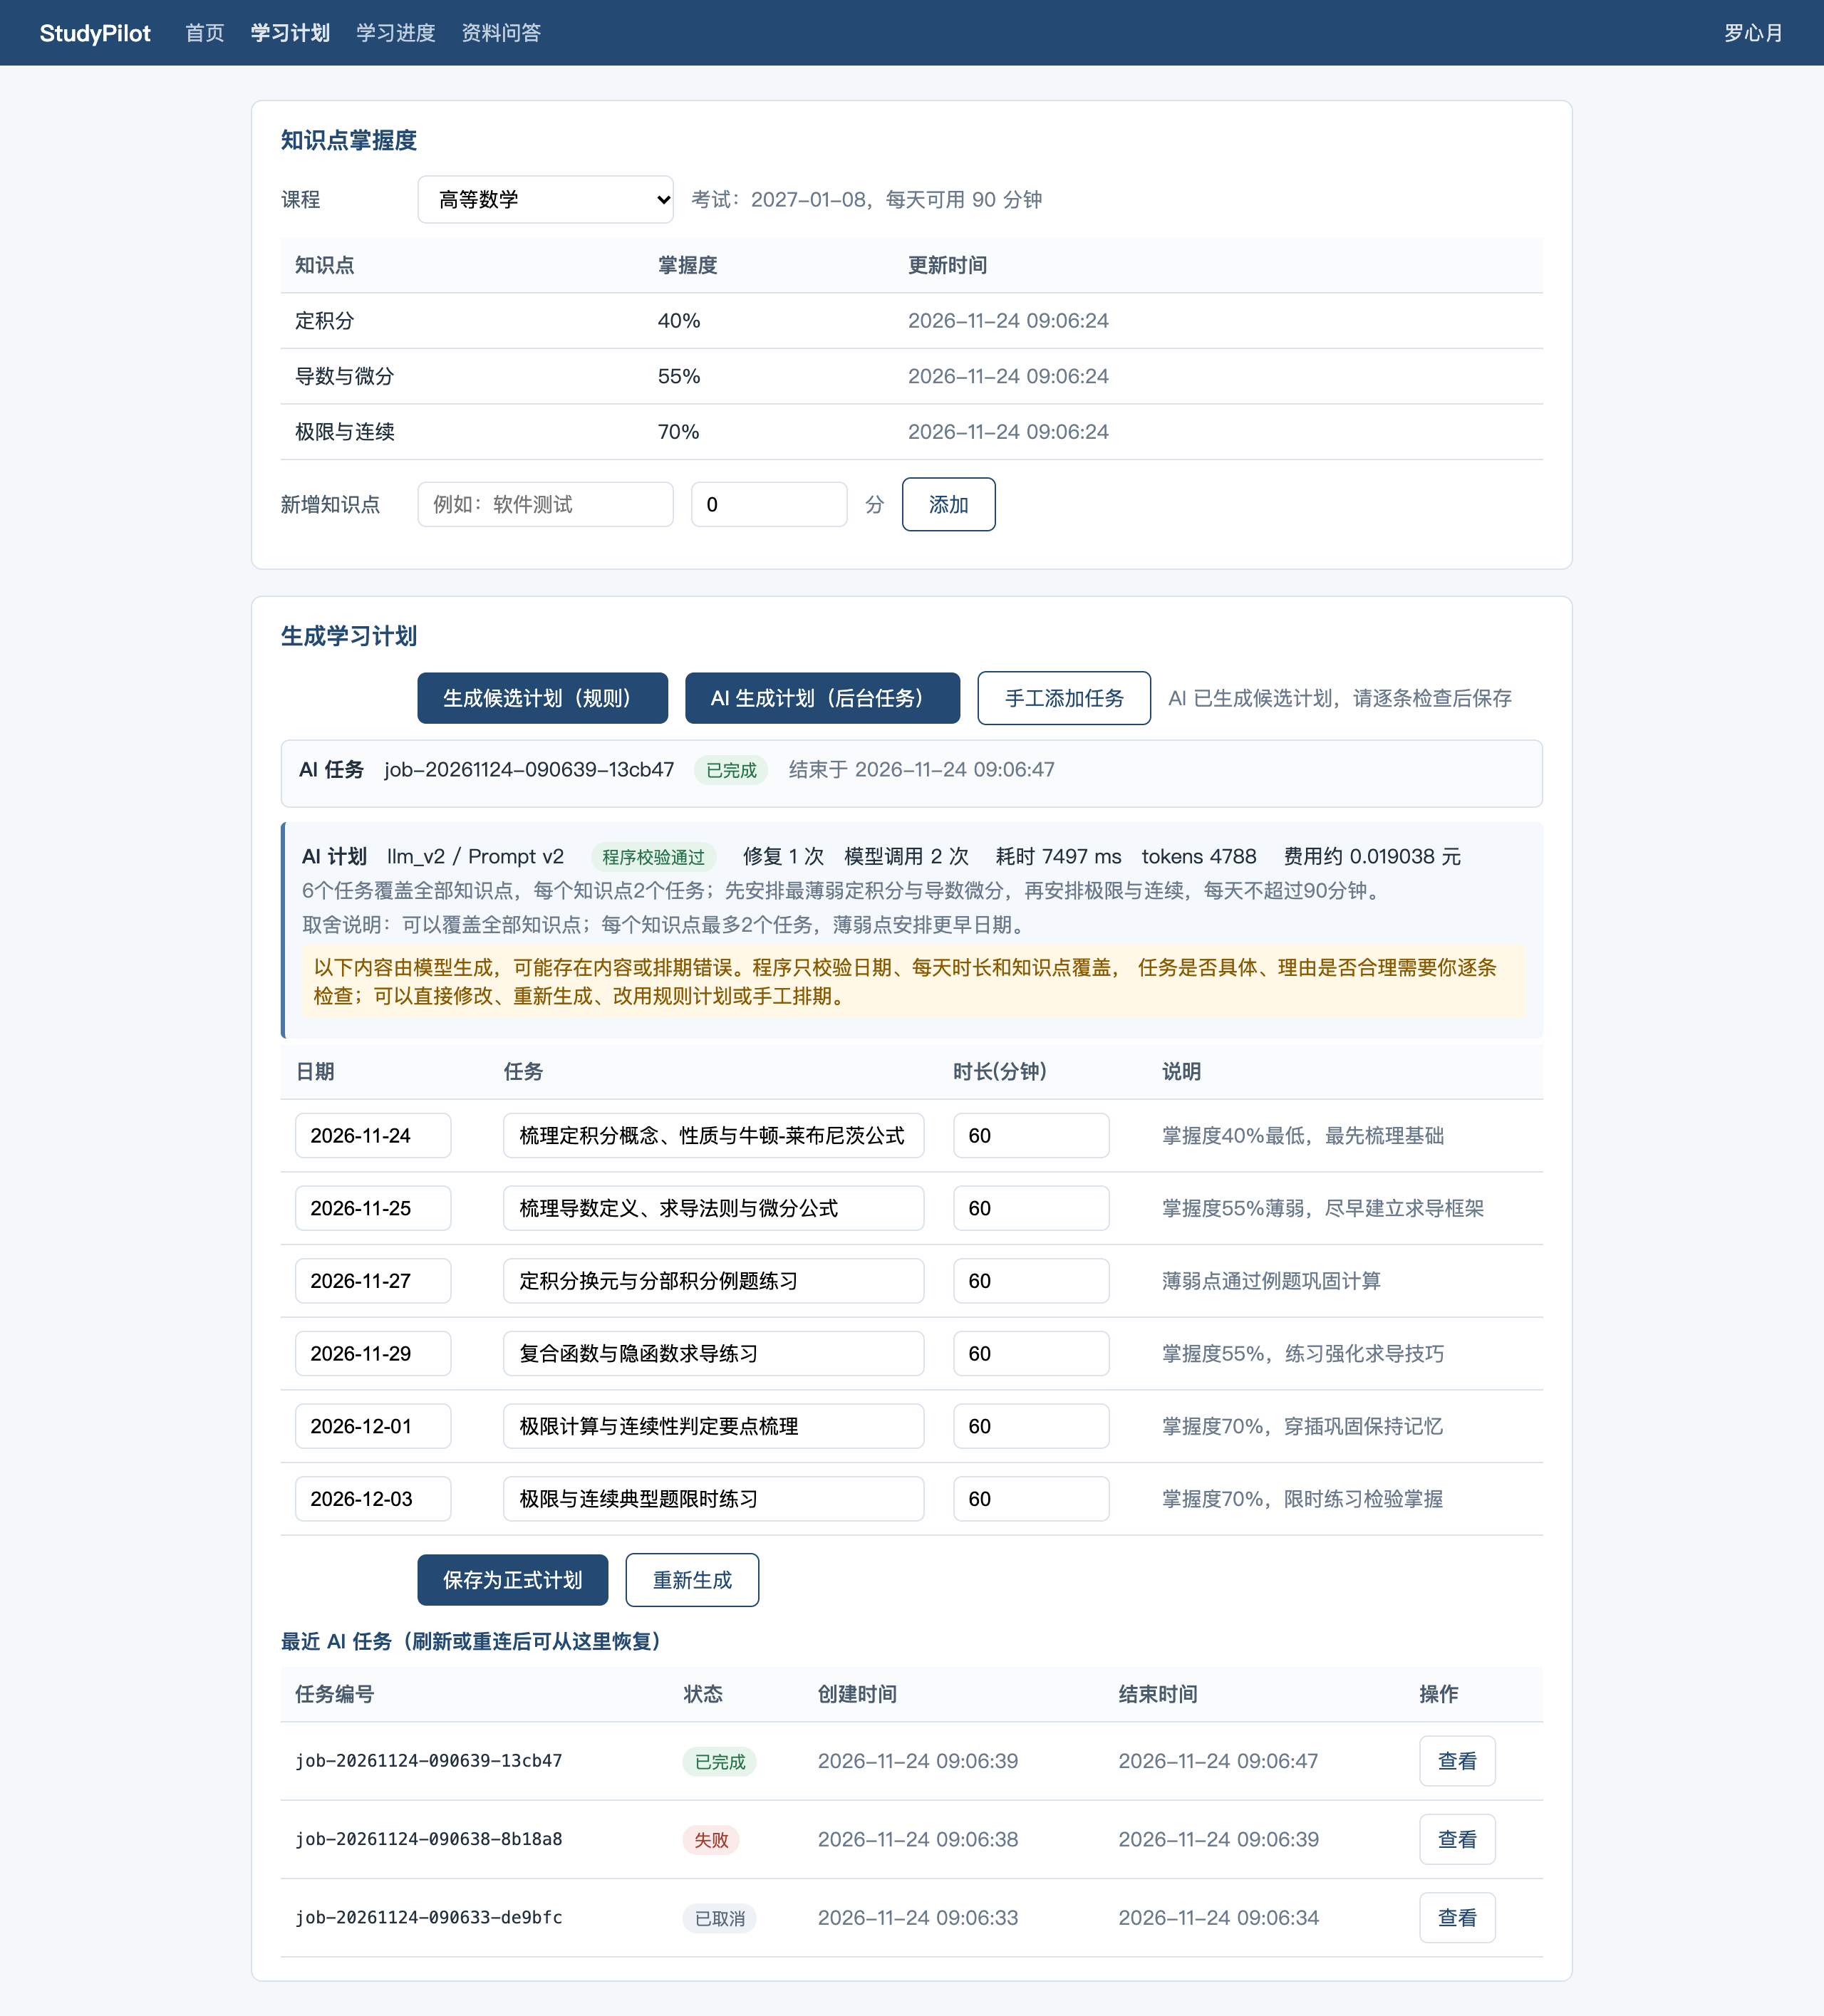
\includegraphics[width=0.92\textwidth]{e8-retry.png}
\caption{重试后成功：新任务编号、结果和保存入口；原失败任务仍保留}
\label{fig:retry}
\end{figure}

图\ref{fig:fallback}演示AI不可用：后端不配置密钥启动，模型调用立即失败（LLM\_NOT\_CONFIGURED），生成器自动降级为规则模板，任务仍然是 succeeded，但结果状态是 fallback，页面明确写“规则模板降级结果（不是模型生成）”，用户仍可编辑保存或稍后重新生成。这满足“用户能够继续操作或安全退出”的要求。除了这种真实的服务不可用，页面 E2E 还用本地故障开关（\texttt{AI\_JOB\_SIMULATION=1} 加 URL 参数 \texttt{sim=timeout/error/slow}）触发超时、连接失败和慢响应，开关默认关闭，正式运行不接受 simulate 参数。

\begin{figure}[htbp]
\centering
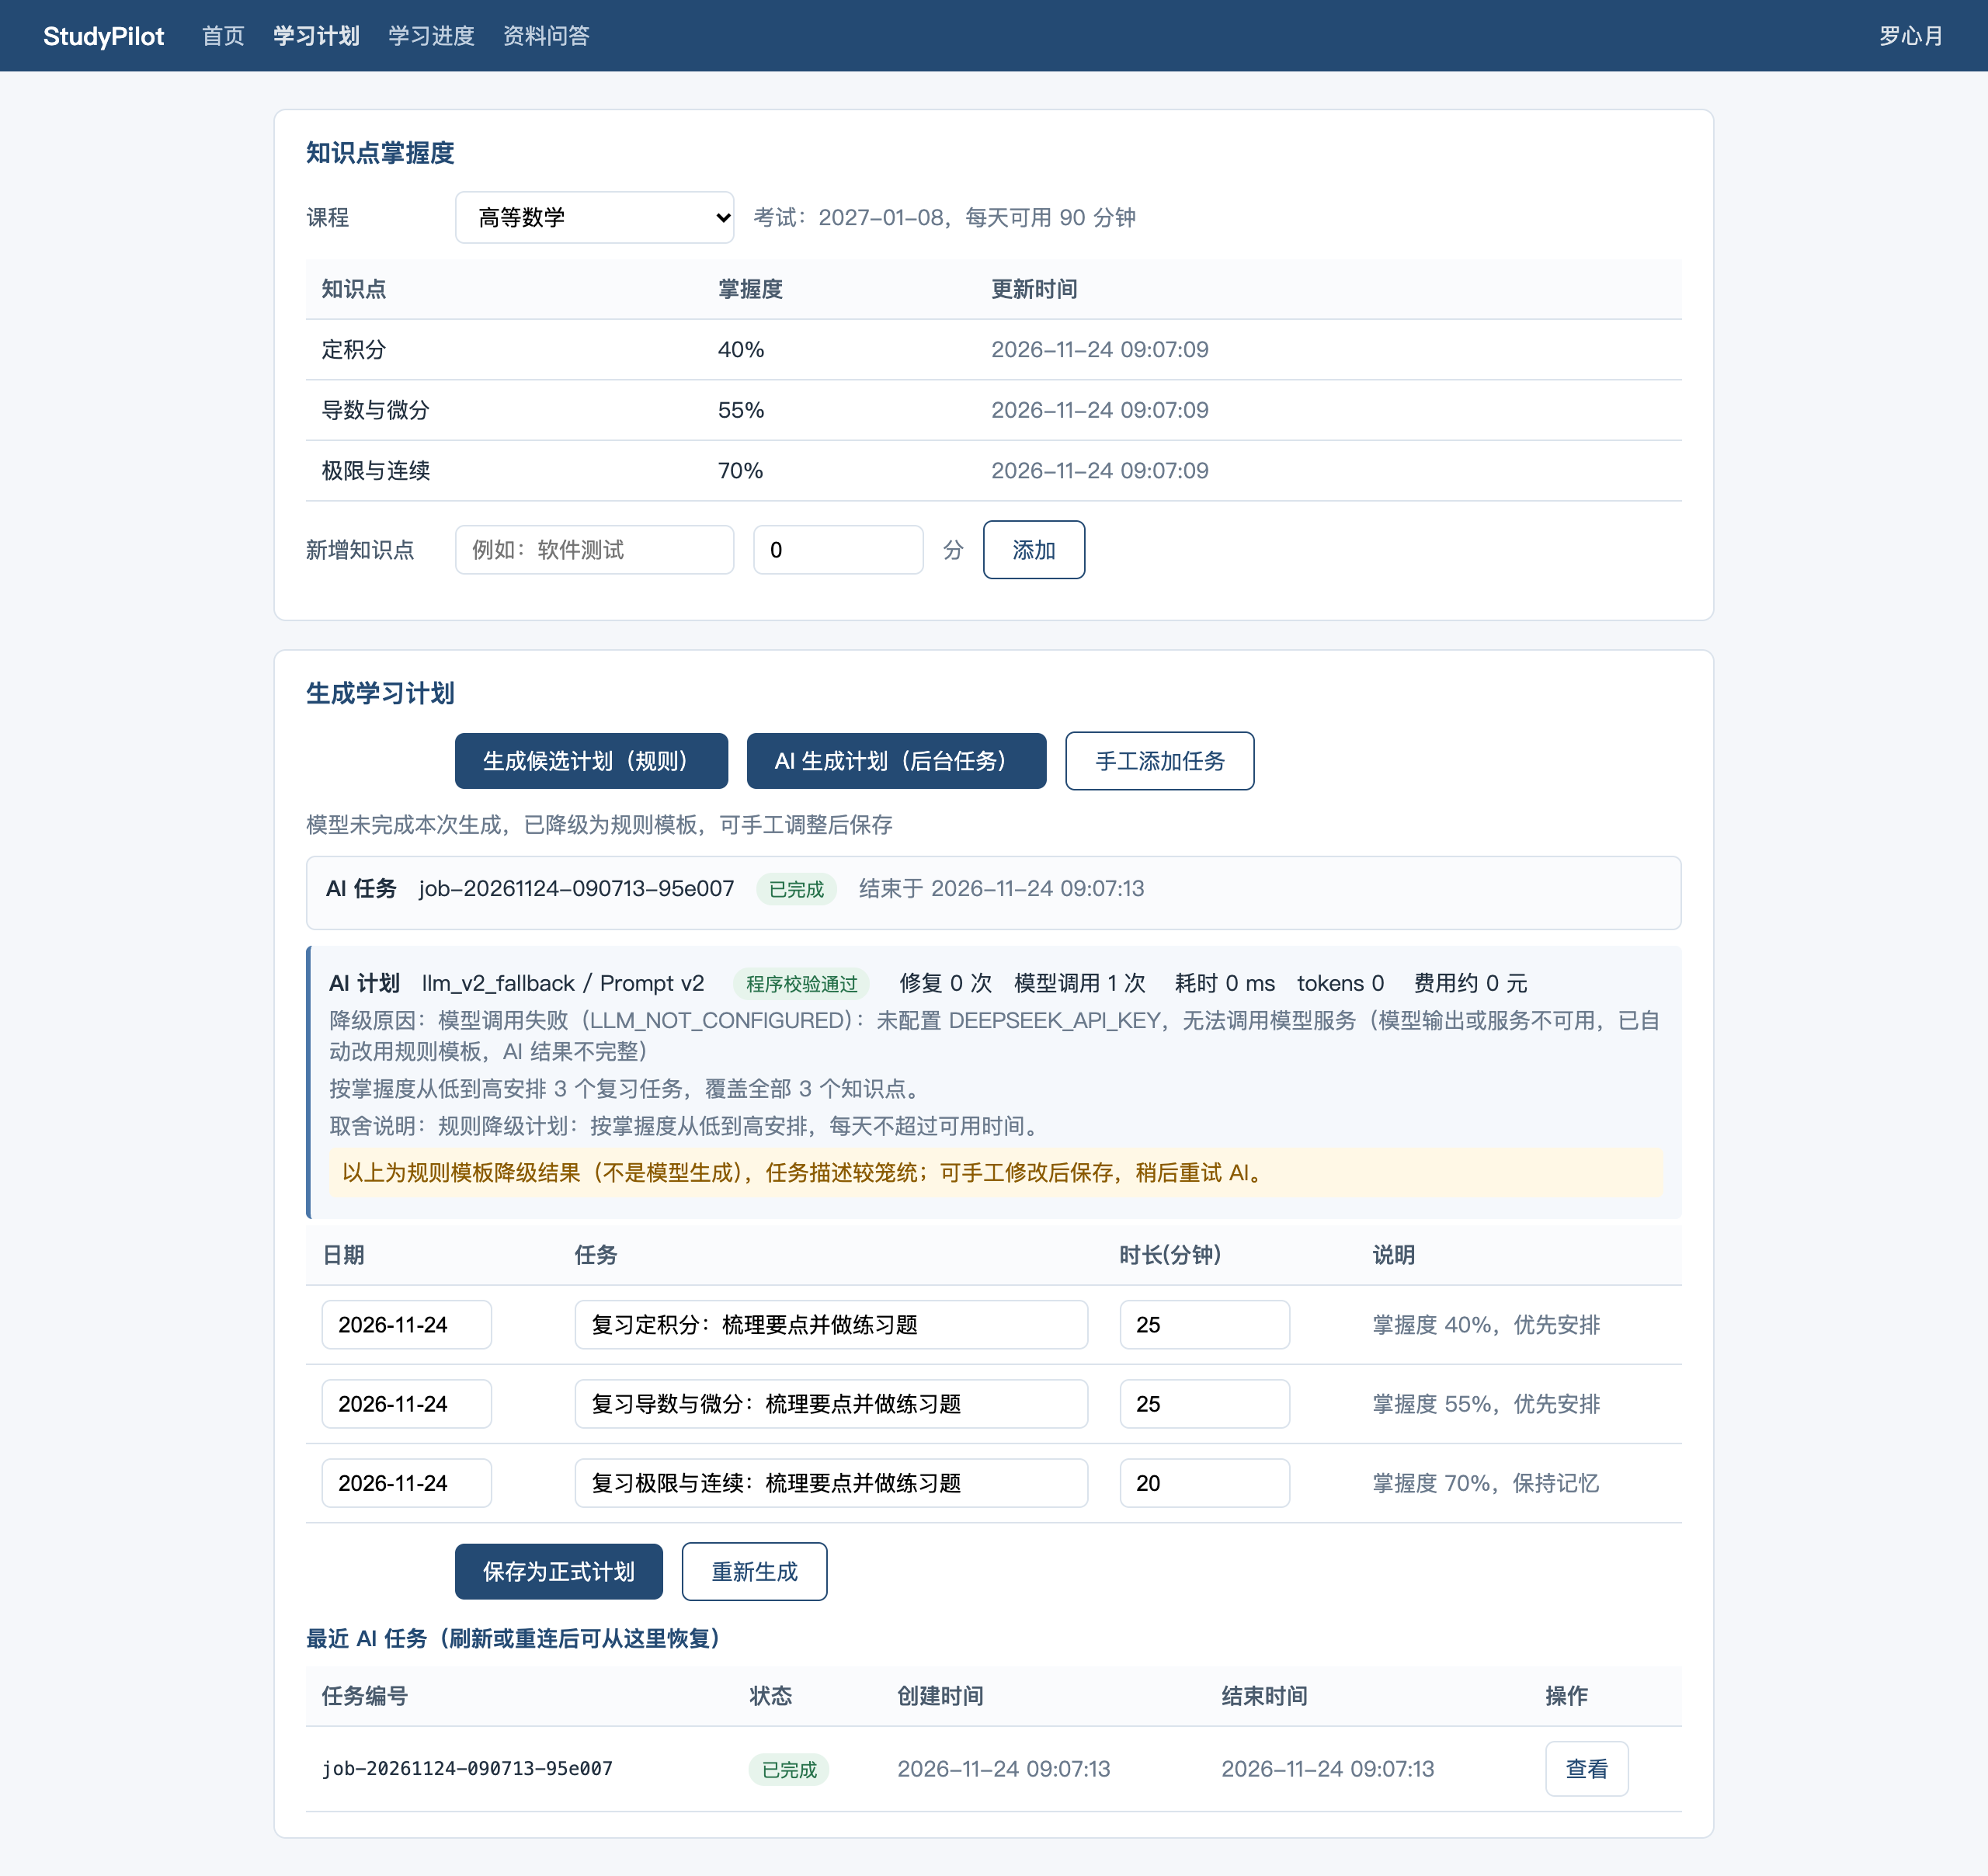
\includegraphics[width=0.92\textwidth]{e8-fallback.png}
\caption{AI不可用降级：未配置密钥时返回规则计划，页面明确标注降级原因和“不是模型生成”}
\label{fig:fallback}
\end{figure}

重试安全性：生成阶段只读数据库、不写计划，因此重试不会产生重复数据；保存阶段只允许 succeeded 且按 \texttt{job\_id} 幂等，重复点击返回同一计划并标记 duplicate；取消后再保存会被 409 拒绝。前端在提交时会生成一次性幂等键并禁用按钮，后端再用“同课程唯一活跃任务 + 幂等键唯一索引”兜底，避免只靠界面限制。

\subsection*{3.5 端到端测试与缺陷修复}

端到端用例覆盖正常、错误输入、等待、取消、失败、重复提交、刷新恢复、交错任务和数据保存，共 14 个，见表\ref{tab:e2e}。页面用例由 \texttt{backend/app/tools/ui\_e2e.py} 用真实 Chrome 操作并断言页面文字，日志在 \texttt{reports/experiment8/runs/e2e-ui.log}；接口用例在 \texttt{backend/tests/test\_integration\_jobs.py}，20 个用例全部离线执行（不调用真实模型），与页面共用同一套接口和状态机。

\begin{table}[H]
\centering
\caption{端到端用例、预期与实际结果}
\label{tab:e2e}
\scriptsize
\begin{tabularx}{\textwidth}{L{1.1cm}L{3.2cm}L{3.5cm}L{3.1cm}X}
\toprule
编号 & 前置与操作 & 预期 & 实际结果 & 证据 \\
\midrule
E2E-01 & 软件工程，点AI生成，等待后编辑一条任务并保存 & 出现任务编号、处理中、完成后可编辑保存 & 正常：3334 ms 完成，保存计划 \#1，编辑内容入库 & 图\ref{fig:wait}--\ref{fig:save} \\
E2E-02 & 提交后观察等待态 & 显示状态和已等待秒数，无百分比 & 显示排队中/处理中、秒数和“可离开”提示 & 图\ref{fig:wait} \\
E2E-03 & 慢响应时点取消，等待迟到结果 & 任务保持已取消，无结果，不能保存 & 取消后 2.5 s 模型返回被丢弃，状态仍 canceled & 图\ref{fig:cancel} \\
E2E-04 & 模拟超时，失败后点重试 & 显示错误和操作入口；重试成功 & LLM\_TIMEOUT 失败；新任务成功（2 次调用、7.5 s） & 图\ref{fig:failed}、\ref{fig:retry} \\
E2E-05 & 执行中刷新页面 & 恢复同一任务并继续轮询 & 刷新后仍等待同一 job，随后成功 & 图\ref{fig:recovery} \\
E2E-06 & 无密钥启动后端，生成计划 & 返回规则降级结果并明确标注 & 任务 succeeded、result.status=fallback、原因可见 & 图\ref{fig:fallback} \\
E2E-07 & 两门课程同时提交，B先返回、A后返回 & 两任务编号不同，内容不混用 & 作业分别完成，任务与知识点各属本课程 & \texttt{e2e-ui.log} 场景5 \\
E2E-08 & 无考试目标课程提交 & 400 GOAL\_NOT\_FOUND，不创建任务 & 返回400，任务列表为空 & \texttt{pytest.log} \\
E2E-09 & 连续/并发提交同一课程 & 返回同一 job\_id，只有一条任务 & 顺序与并发都复用任务，无500 & \texttt{pytest.log} \\
E2E-10 & 同一幂等键重复提交 & 返回已有任务，不重复调用模型 & 成功任务被复用，标记 deduplicated & \texttt{pytest.log} \\
E2E-11 & 成功后保存两次；另用编辑后的任务保存 & 同一计划、一次写入；编辑生效 & duplicate=true、计划数1；编辑标题与时长入库 & \texttt{pytest.log} \\
E2E-12 & 未结束任务模拟服务重启 & 标记 JOB\_INTERRUPTED，可重新生成 & 状态 failed、错误码正确 & \texttt{pytest.log} \\
E2E-13 & 取消/失败任务点保存；成功任务点重试 & 409，不写计划 & JOB\_NOT\_SUCCEEDED / JOB\_NOT\_RETRYABLE & \texttt{pytest.log} \\
E2E-14 & 把任务结束时间改到10天前并清理 & 超过7天的结束任务被删除，活跃任务保留 & 删除1条，查询返回404 & \texttt{pytest.log} \\
\bottomrule
\end{tabularx}
\end{table}

自动化测试共 83 个全部通过（图\ref{fig:tests}），其中实验8新增 20 个，覆盖正常提交、输入校验、重复提交（含并发）、幂等键、取消、迟到结果、失败重试、降级结果、刷新恢复、启动中断、交错任务、保存幂等、编辑校验和保留期清理。原有的实验4--7测试全部重跑通过，没有因为新增任务层破坏已有功能。

\begin{figure}[htbp]
\centering
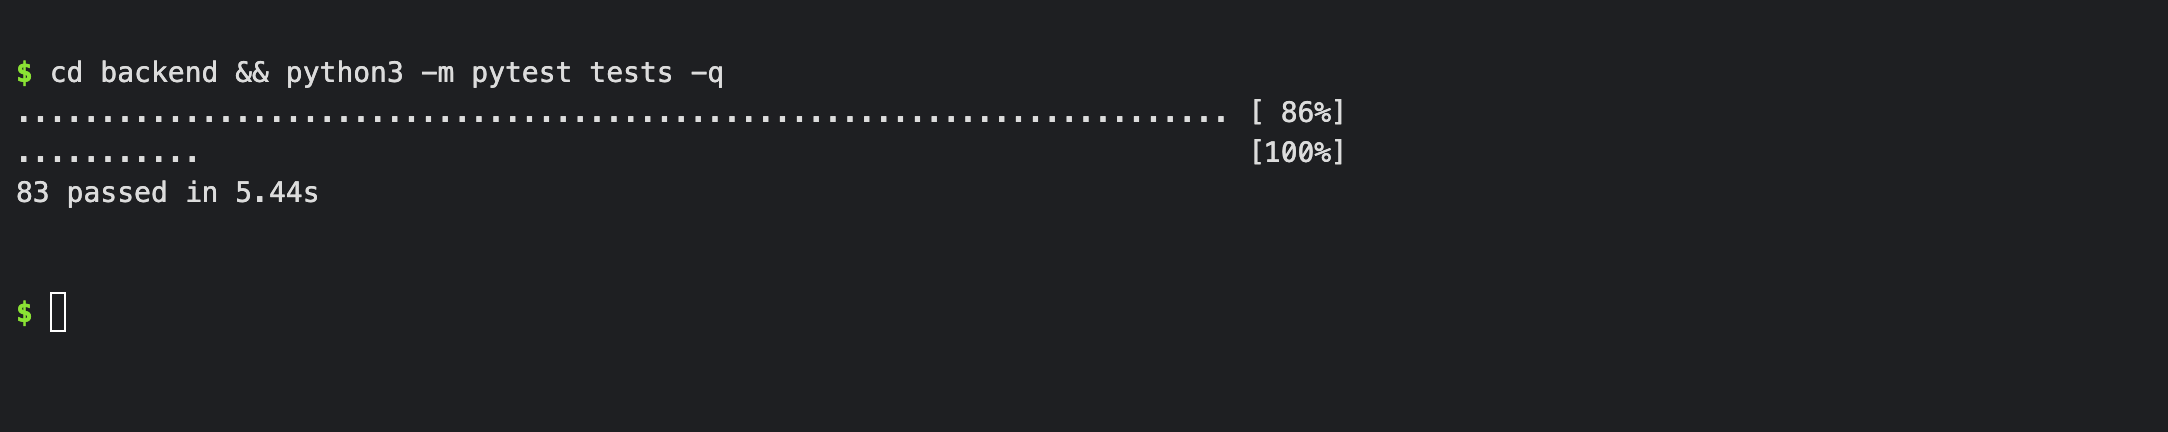
\includegraphics[width=\textwidth]{e8-tests.png}
\caption{全量测试：83 passed；实验8新增 20 个集成用例，原有用例全部通过}
\label{fig:tests}
\end{figure}

\begin{figure}[htbp]
\centering
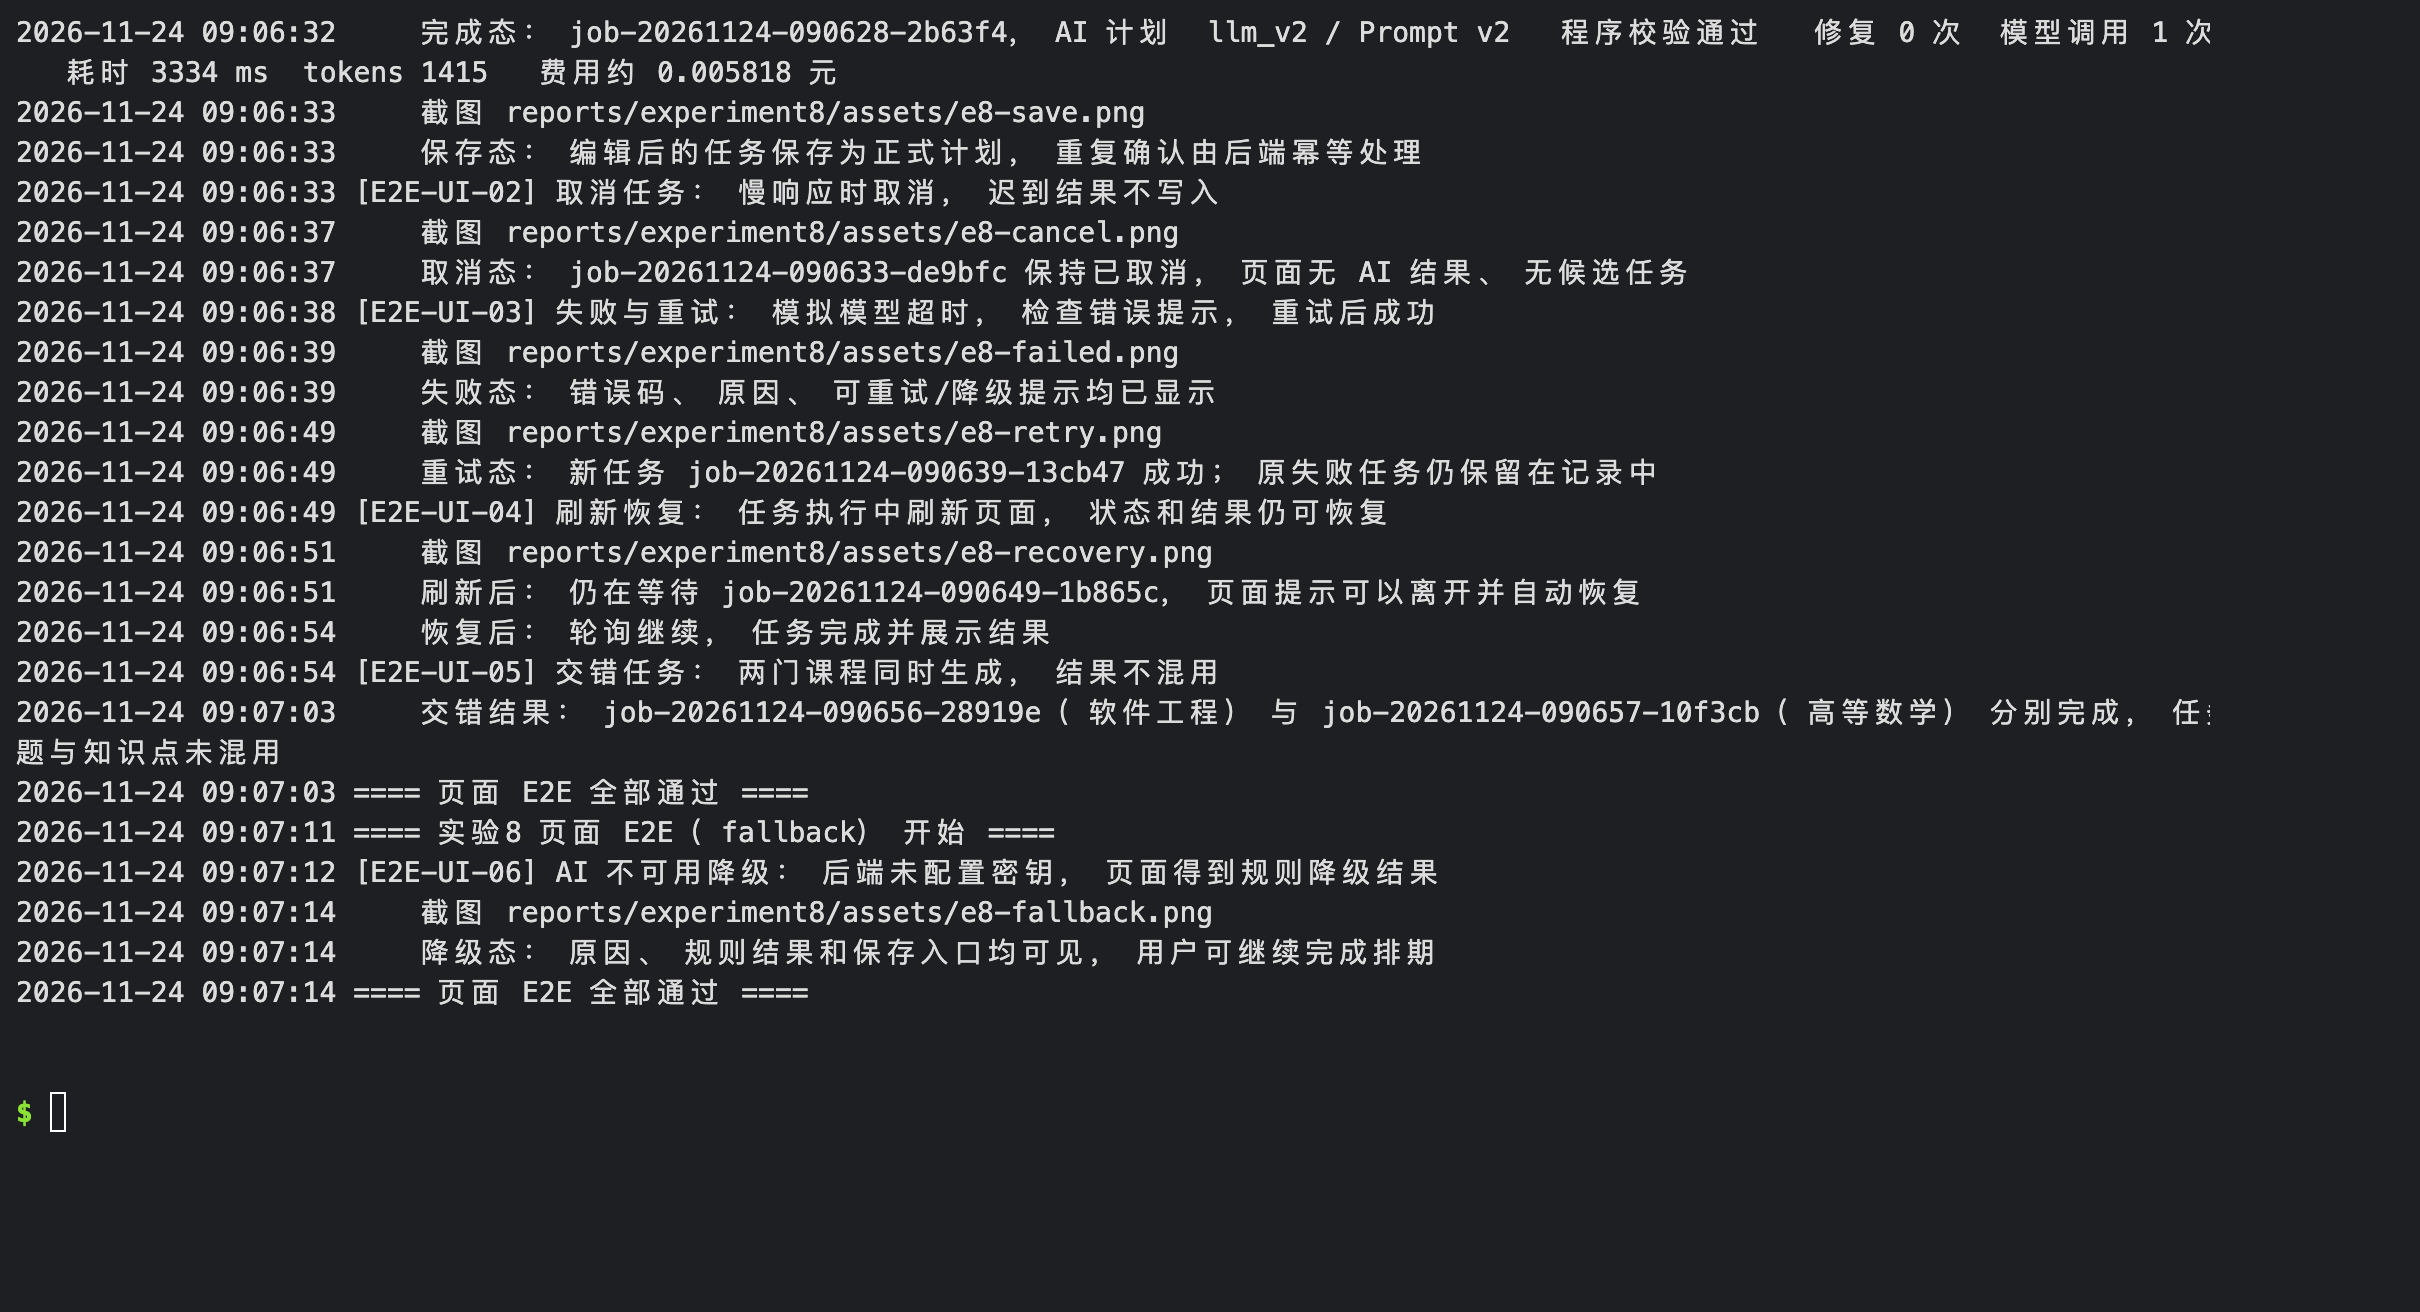
\includegraphics[width=\textwidth]{e8-e2e-log.png}
\caption{页面端到端日志：6 个场景全部通过，含任务编号、完成耗时与截图路径}
\label{fig:e2elog}
\end{figure}

本次开发中实际发现并修复的缺陷见表\ref{tab:defects}。四个缺陷都影响真实使用，修复后分别用自动化测试、页面 E2E 或手工复现验证；修复代码包含在提交 \texttt{443304b}（tag v0.7）中。

\begin{table}[H]
\centering
\caption{实际发现的缺陷、修复与复测}
\label{tab:defects}
\scriptsize
\begin{tabularx}{\textwidth}{L{0.9cm}L{2.9cm}L{2.4cm}L{3.1cm}L{2.2cm}X}
\toprule
编号 & 影响与复现 & 可能原因 & 修复 & 复测 & 修复Commit \\
\midrule
D8-01 & 双击/并发提交时第二个请求可能返回500“数据库暂时不可用”，用户以为服务故障 & 唯一索引冲突被通用数据库异常包装，未识别为重复提交 & 插入时单独捕获 IntegrityError，改为查询并复用已有活跃任务 & 顺序与并发重复提交用例均返回同一 job\_id & \texttt{443304b} \\
D8-02 & 无密钥降级后页面仍显示“AI 计划/程序校验通过”，容易被误认为模型结果 & 结果区文案固定，未区分 success 与 fallback & 降级时单独提示“规则模板降级结果（不是模型生成）” & 无密钥页面 E2E 断言降级文案通过 & \texttt{443304b} \\
D8-03 & 已在学习计划页时从链接切到另一门课程，页面仍显示上一门课程的数据 & 页面只在挂载时读一次 \texttt{route.query.course}，路由复用组件不重新挂载 & 监听 query 变化并重新加载课程数据 & 切换课程检查与 E2E 交错用例通过 & \texttt{443304b} \\
D8-04 & 某任务处理中时点历史任务的“查看”，当前任务不再轮询，等待状态像丢失 & 历史列表“查看”未限制处理中的切换 & 处理中禁用其他任务的“查看”，只保留当前任务轮询 & 恢复场景截图与刷新恢复用例通过 & \texttt{443304b} \\
\bottomrule
\end{tabularx}
\end{table}

缺陷之外的检查范围：并发保存（同一任务两次 confirm）通过 \texttt{\_confirm\_lock} 和 \texttt{confirmed\_plan\_id} 条件更新保证只写一次；数据库不可用时任务创建返回 500 并记录日志，已保存计划不受影响；密钥只从环境变量读取，日志和报告中未出现完整密钥；前端构建与后端全量测试均通过。

\subsection*{3.6 试用}

试用固定使用 v0.7、\texttt{deepseek-chat}、Prompt v2，浏览器为 Chrome，前后端按 README 启动。只向试用者提供正常操作说明和三条任务，不演示、不代为操作、不解释实现；试用记录在 \texttt{reports/experiment8/runs/trial.json}，参与者为同班同学（非开发者，应要求匿名）。第一轮完成后按反馈修改，再邀请同一人做第二轮。试用任务与结果见表\ref{tab:trial}。

\begin{table}[H]
\centering
\caption{试用任务、完成情况与两轮变化}
\label{tab:trial}
\small
\begin{tabularx}{\textwidth}{L{0.9cm}L{4.6cm}L{1.2cm}L{1.4cm}L{1.4cm}X}
\toprule
编号 & 任务 & 完成 & 第1轮用时 & 第2轮用时 & 观察 \\
\midrule
T1 & 为高等数学生成AI计划并保存 & 是 & 2分48秒 & 1分35秒 & 第一轮在等待态停留较久，担心离开会丢；第二轮看到“可以离开本页”后直接等待 \\
T2 & 生成过程中刷新，确认任务不丢 & 是 & 1分14秒 & 48秒 & 第一轮刷新后想重新点生成；第二轮会从“最近AI任务”恢复 \\
T3 & 取消一次生成，改用规则计划保存 & 是 & 1分01秒 & 52秒 & 第一轮先点重试又取消，走了弯路；第二轮直接取消后改用规则生成 \\
\midrule
\multicolumn{2}{r}{三条任务合计} & 3/3 & 约5分03秒 & 约3分15秒 & 两轮均无代操作、无提示 \\
\bottomrule
\end{tabularx}
\end{table}

第一轮的主要困惑：(1)“排队中”和“处理中”同时可能出现，不知道是在排队还是模型卡住；(2)按钮变成“AI 任务处理中…”后以为整个页面被锁住；(3)降级结果仍写“AI 计划/程序校验通过”，误以为是模型结果；(4)任务处理中点了历史“查看”，当前等待状态不再更新；(5)任务标题输入框太窄，长标题看不全。对应的修改是：状态行区分排队/处理中并显示已等待秒数、提示可以离开和刷新恢复；按钮文案改为“AI 生成中…”；降级结果单独标注“不是模型生成”；处理中禁用其他历史任务的“查看”；加宽标题输入框并显示任务结束时间。第二轮三条任务都能独立完成，困惑减少，剩余意见是希望看到每次模型调用的费用明细（当前只显示总费用，作为后续改进）。试用是单人小样本，不能代表所有用户；报告把它作为可用性参考，而不是统计结论。

\subsection*{3.7 版本对比}

课程安排上实验7对应第1周的原型（v0.6），实验8对应第2周的集成（v0.7）。两次提交的实际时间都在 2026-11-24 上午（v0.6 为 08:27，v0.7 为 09:08），是课程压缩后的连续验收，报告不把它描述成真实相隔两周；比较的是同一门课程、同一模型、同一生成器下的两种软件集成方式。功能对比见表\ref{tab:version}，实测数据见表\ref{tab:metrics}，v0.6 页面见图\ref{fig:v06}。

\begin{table}[H]
\centering
\caption{v0.6 同步入口与 v0.7 任务式集成的功能对比}
\label{tab:version}
\small
\begin{tabularx}{\textwidth}{L{3.0cm}L{5.7cm}X}
\toprule
对比项 & v0.6（实验7，69cc0be/tag v0.6） & v0.7（实验8，443304b/tag v0.7） \\
\midrule
页面入口 & “AI 生成计划（带检查）”，同步等待 & “AI 生成计划（后台任务）”，提交后立即返回 \\
任务状态 & 只有按钮“生成中…”，无任务编号 & queued/running/succeeded/failed/canceled + 最近任务列表 \\
取消 & 不支持 & 支持；停止等待，迟到结果丢弃 \\
刷新/重启恢复 & 刷新即丢失 & 页面恢复最近任务；重启遗留任务标记中断 \\
重复提交 & 重复点击会重复调用模型 & 同课程唯一活跃任务 + 幂等键，直接复用 \\
失败处理 & 一次HTTP错误或自动降级，页面只显示当前结果 & 失败任务保留错误码、提示、重试；降级单独标注 \\
保存 & 直接确认写计划，无任务级幂等 & 只允许成功任务保存，按 job\_id 幂等 \\
测试 & 全套63个（实验7 20个） & 全套83个（新增20个集成用例 + 6个页面场景） \\
\bottomrule
\end{tabularx}
\end{table}

\begin{figure}[htbp]
\centering
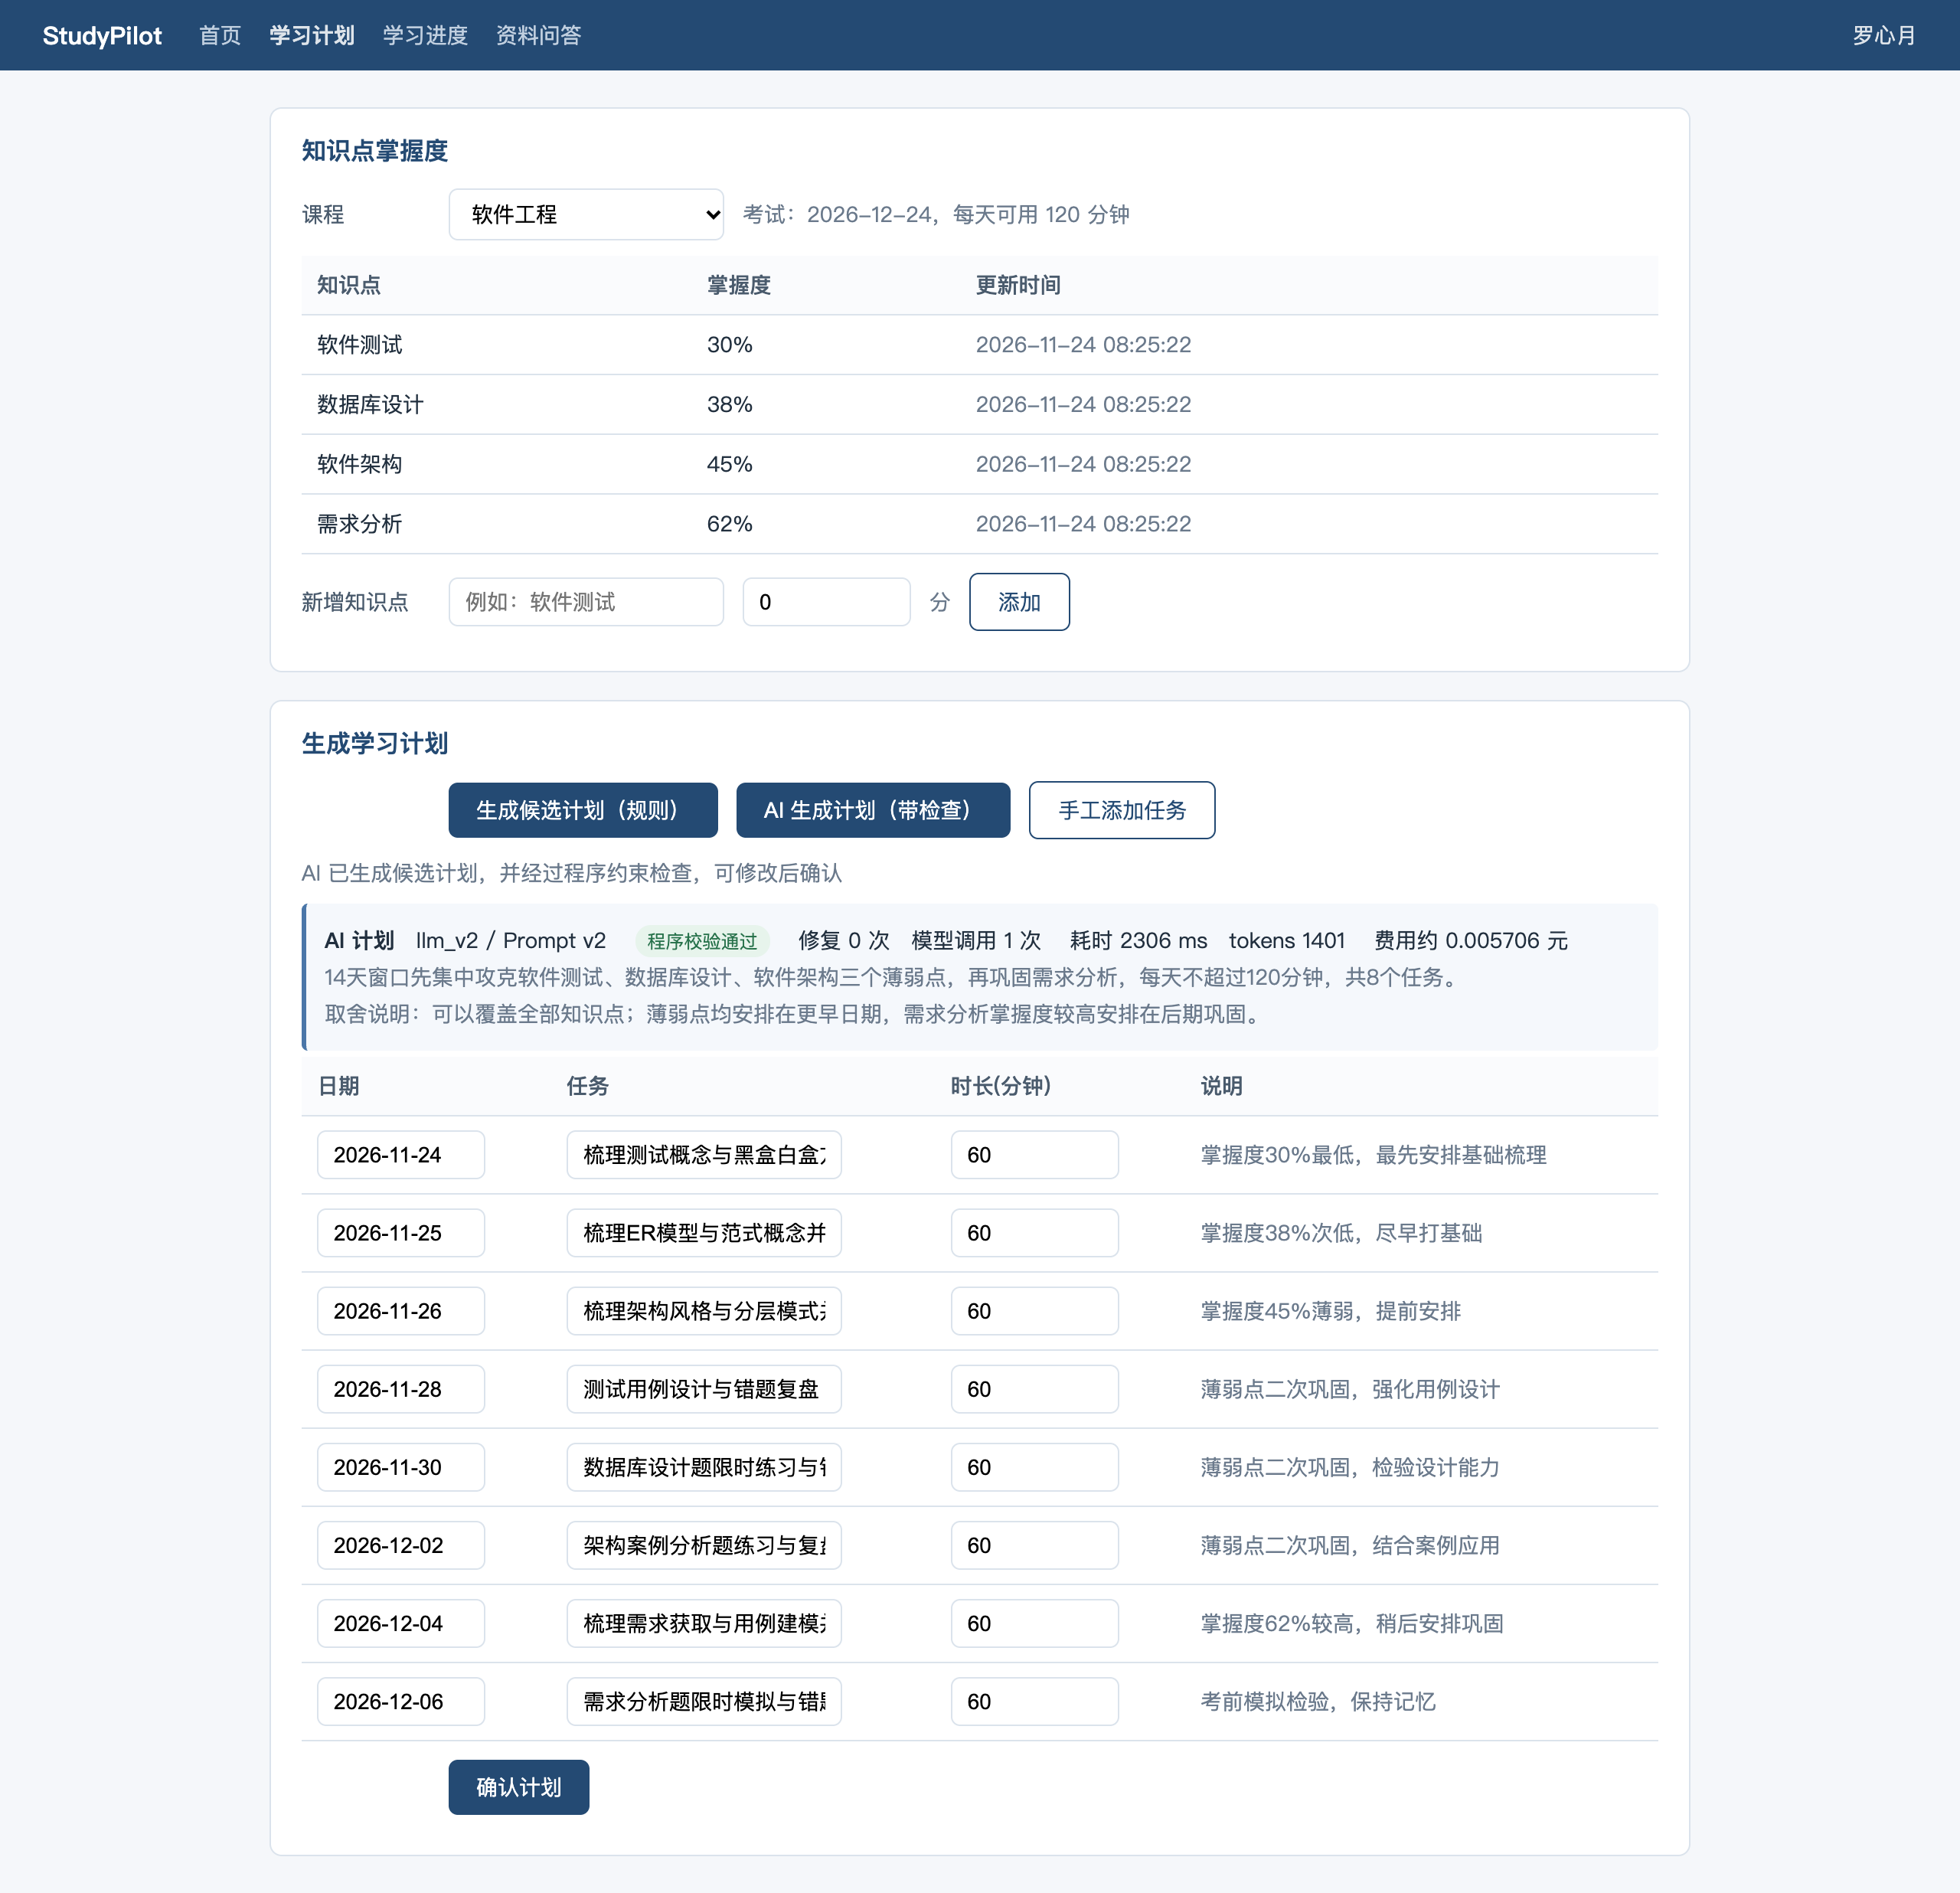
\includegraphics[width=0.9\textwidth]{e8-v06-ui.png}
\caption{v0.6页面：只有同步“AI 生成计划（带检查）”，没有任务编号、状态、取消和历史}
\label{fig:v06}
\end{figure}

同一门课程、同一模型各跑3次，v0.6 与 v0.7 的实测对比见表\ref{tab:metrics}。v0.6 的“提交响应”就是完整生成时间（平均 7.1 秒，最长 8.8 秒），v0.7 提交平均 5.7 毫秒，用户马上看到任务编号；两者总生成时间接近（v0.7 平均 6.95 秒），说明任务化没有让模型变慢或变快，改变的是用户能否在等待中操作和失败后恢复。v0.6 三次中有一次模型输出未通过、返回 fallback；v0.7 三次都是 success，但样本只有3次，且两版使用同一生成器和 Prompt，不能据此说v0.7的AI质量更高，只能说明集成层没有改变生成结果。

\begin{table}[H]
\centering
\caption{同课程同模型的集成方式实测（各3次，2026-11-24）}
\label{tab:metrics}
\small
\begin{tabularx}{\textwidth}{L{4.2cm}L{4.6cm}X}
\toprule
指标 & v0.6 同步 & v0.7 任务式 \\
\midrule
提交响应时间 & 平均 7118 ms（4875--8798） & 平均 5.7 ms（5--7），立即返回 job\_id \\
总生成时间 & 平均 7118 ms & 平均 6955 ms（3468--11590，含排队与轮询） \\
任务完成情况 & 3/3 程序检查通过，1次 fallback & 3/3 成功，程序检查通过 \\
取消/离开页面 & 不支持，离开即失去等待 & 支持，页面可离开/刷新，任务继续 \\
重复提交 & 会重复调用模型 & 同课程唯一活跃任务，第二次返回原任务 \\
失败后恢复 & 重新点击，无状态可查 & 失败任务可重试；取消/失败可改用规则计划 \\
\bottomrule
\end{tabularx}
\end{table}

结论是：本次集成的价值不在“让模型更快”，而在把一次不可控的长请求变成有编号、有状态、可取消、可恢复、可保存的任务；同时把模型失败纳入软件的错误与降级流程，用户在AI不可用时仍能完成排期。v0.6 的同步接口保留在代码中，作为对照，不影响新页面。

\subsection*{3.8 关键代码}

任务状态转换集中在 \texttt{app/service/job\_service.py} 的 \texttt{execute\_job}（代码\ref{lst:execute}）：先尝试把 queued 改为 running，再执行生成；返回后检查取消标志，只有未取消才写成功结果，异常则写失败；取消后迟到的结果直接丢弃。

\begin{lstlisting}[caption={后台执行与迟到结果处理},label={lst:execute}]
def execute_job(job_id: str) -> None:
    job = job_repo.get(job_id)
    if not job or job["status"] != "queued":
        return
    if not job_repo.mark_running(job_id):
        return
    try:
        result = generator.generate(...)
        if job_repo.get(job_id)["cancel_requested"]:
            joblog.event(job_id, "late_result_discarded", ...)
            return
        if not job_repo.mark_succeeded(job_id, json.dumps(result, ensure_ascii=False)):
            joblog.event(job_id, "late_result_discarded", ...)
            return
    except BusinessError as exc:
        if job_repo.get(job_id)["cancel_requested"]:
            joblog.event(job_id, "late_error_discarded", error_code=exc.code)
            return
        job_repo.mark_failed(job_id, exc.code, exc.message)
\end{lstlisting}

保存的幂等处理见代码\ref{lst:confirm}：先看任务是否已有 confirmed\_plan\_id，有则直接返回同一计划；没有则只接受 succeeded，校验用户编辑后的任务，再在锁内写入并回填关联，重复确认不会生成第二份计划。

\begin{lstlisting}[caption={保存结果的任务级幂等},label={lst:confirm}]
def confirm_job(job_id: str, tasks=None) -> dict:
    job = _get_or_404(job_id)
    if job.get("confirmed_plan_id"):
        return {"plan_id": job["confirmed_plan_id"], "duplicate": True, ...}
    if job["status"] != "succeeded":
        raise BusinessError("只有生成成功的任务才能保存", 409, "JOB_NOT_SUCCEEDED")
    tasks = _validate_tasks(tasks if tasks is not None else result.get("tasks"))
    with _confirm_lock:
        job = _get_or_404(job_id)
        if job.get("confirmed_plan_id"):
            return {"plan_id": job["confirmed_plan_id"], "duplicate": True, ...}
        plan = plan_service.confirm_plan(job["course_id"], tasks, generator=...)
        job_repo.set_confirmed_plan(job_id, plan["plan_id"])
        return {**plan, "duplicate": False}
\end{lstlisting}

前端轮询见代码\ref{lst:poll}：提交后只保存 job\_id，1.2 秒轮询一次；状态到终态就停止计时，成功时恢复任务列表，失败/取消显示对应入口；查询失败时保留当前状态并继续重试，不把网络抖动当成任务失败。

\begin{lstlisting}[caption={页面轮询与终态处理（Vue 3）},label={lst:poll}]
async function poll() {
  const data = await getPlanJob(job.value.job_id)
  const wasActive = jobActive.value
  job.value = data
  if (wasActive && !jobActive.value) {
    clearTimers()
    if (data.status === 'succeeded') restoreTasks(data.result)
    if (data.status === 'failed') notice.value = ''
    await refreshJobList()
    return
  }
  schedulePoll()
}
\end{lstlisting}

\subsection*{3.9 版本记录与仓库}

代码、测试、说明和运行记录保存在个人 GitHub 仓库 \url{https://github.com/luohao711/StudyPilot}。实验8的实现提交为 \texttt{443304b}（tag \texttt{v0.7}），实验7对照版本为 \texttt{69cc0be}（tag \texttt{v0.6}）；提交记录、推送结果和仓库页面分别见图\ref{fig:gitlog}、图\ref{fig:push}、图\ref{fig:github}。本报告、截图和运行记录在实现提交之后随报告提交一并入库，报告中的文件路径均可在仓库 \texttt{reports/experiment8/} 下复核。

\begin{figure}[htbp]
\centering
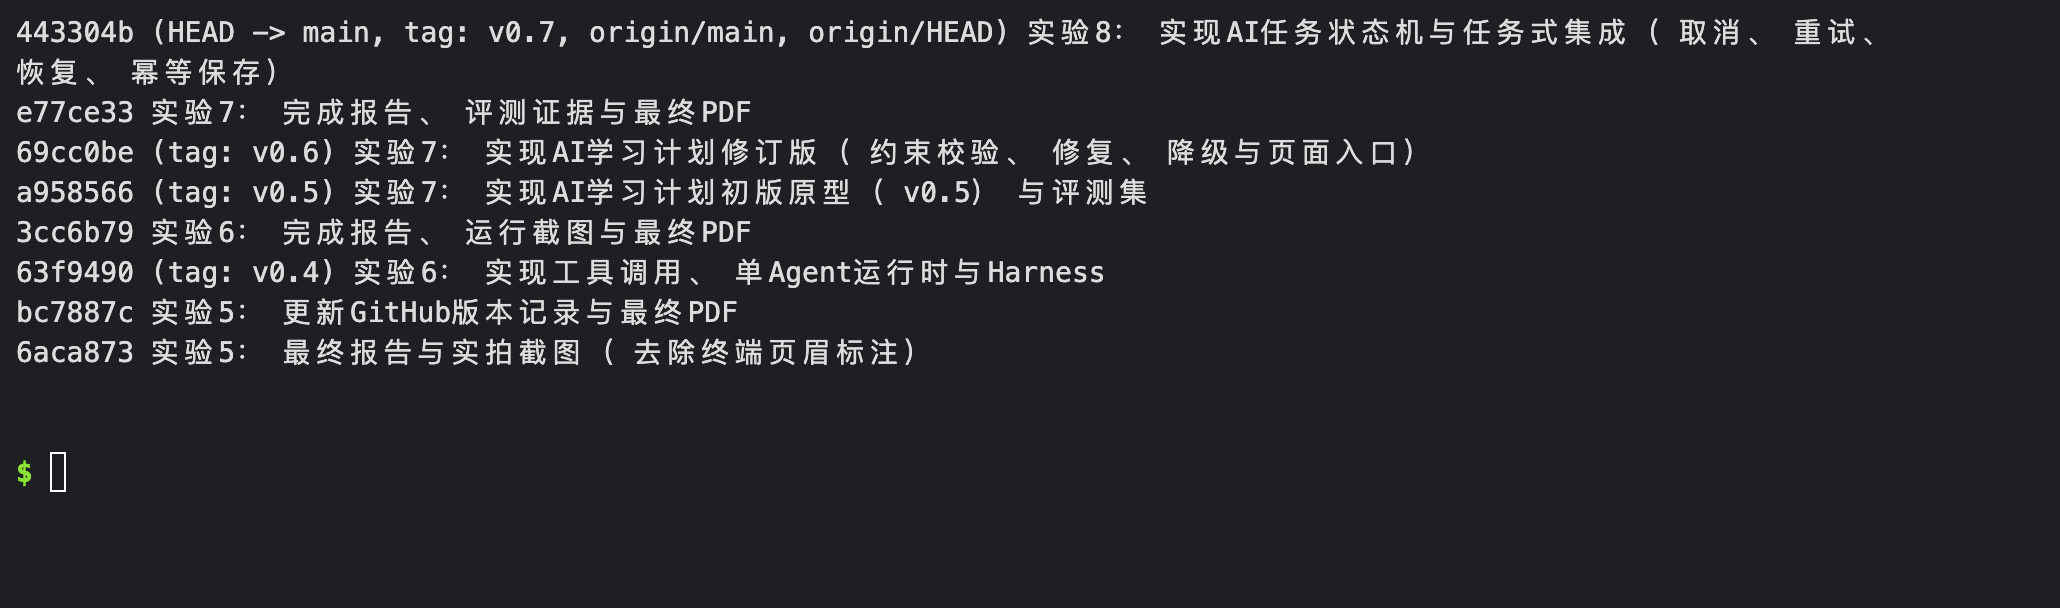
\includegraphics[width=\textwidth]{e8-gitlog.png}
\caption{Git 提交记录：443304b（tag v0.7）为实验8实现提交，69cc0be（tag v0.6）为实验7对照版本}
\label{fig:gitlog}
\end{figure}

\begin{figure}[htbp]
\centering
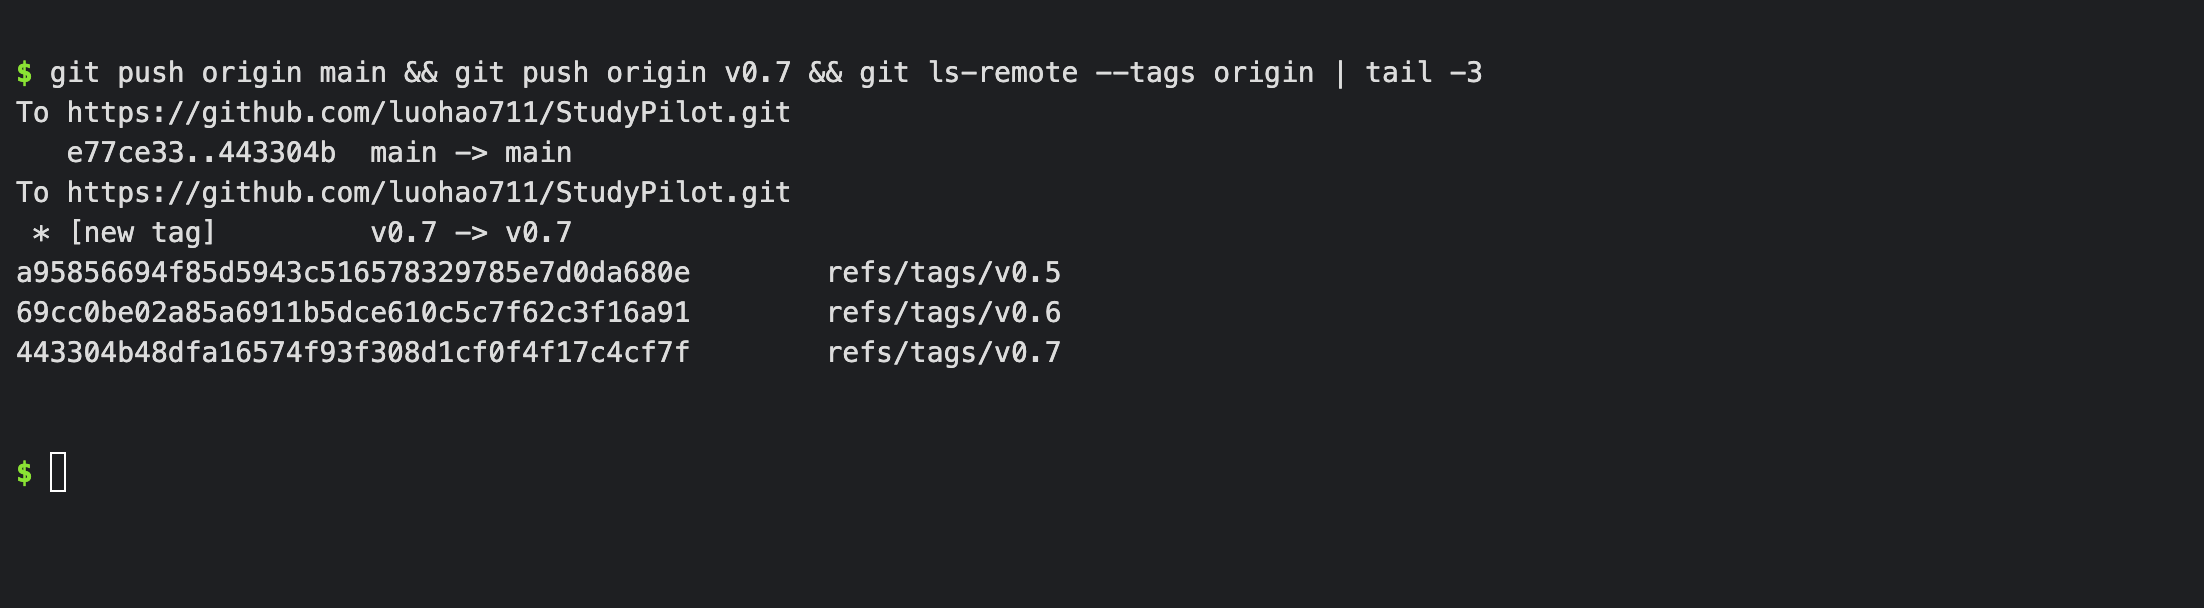
\includegraphics[width=\textwidth]{e8-push.png}
\caption{推送 main 与 tag v0.7；远端已有 v0.5、v0.6、v0.7 三个版本标签}
\label{fig:push}
\end{figure}

\begin{figure}[htbp]
\centering
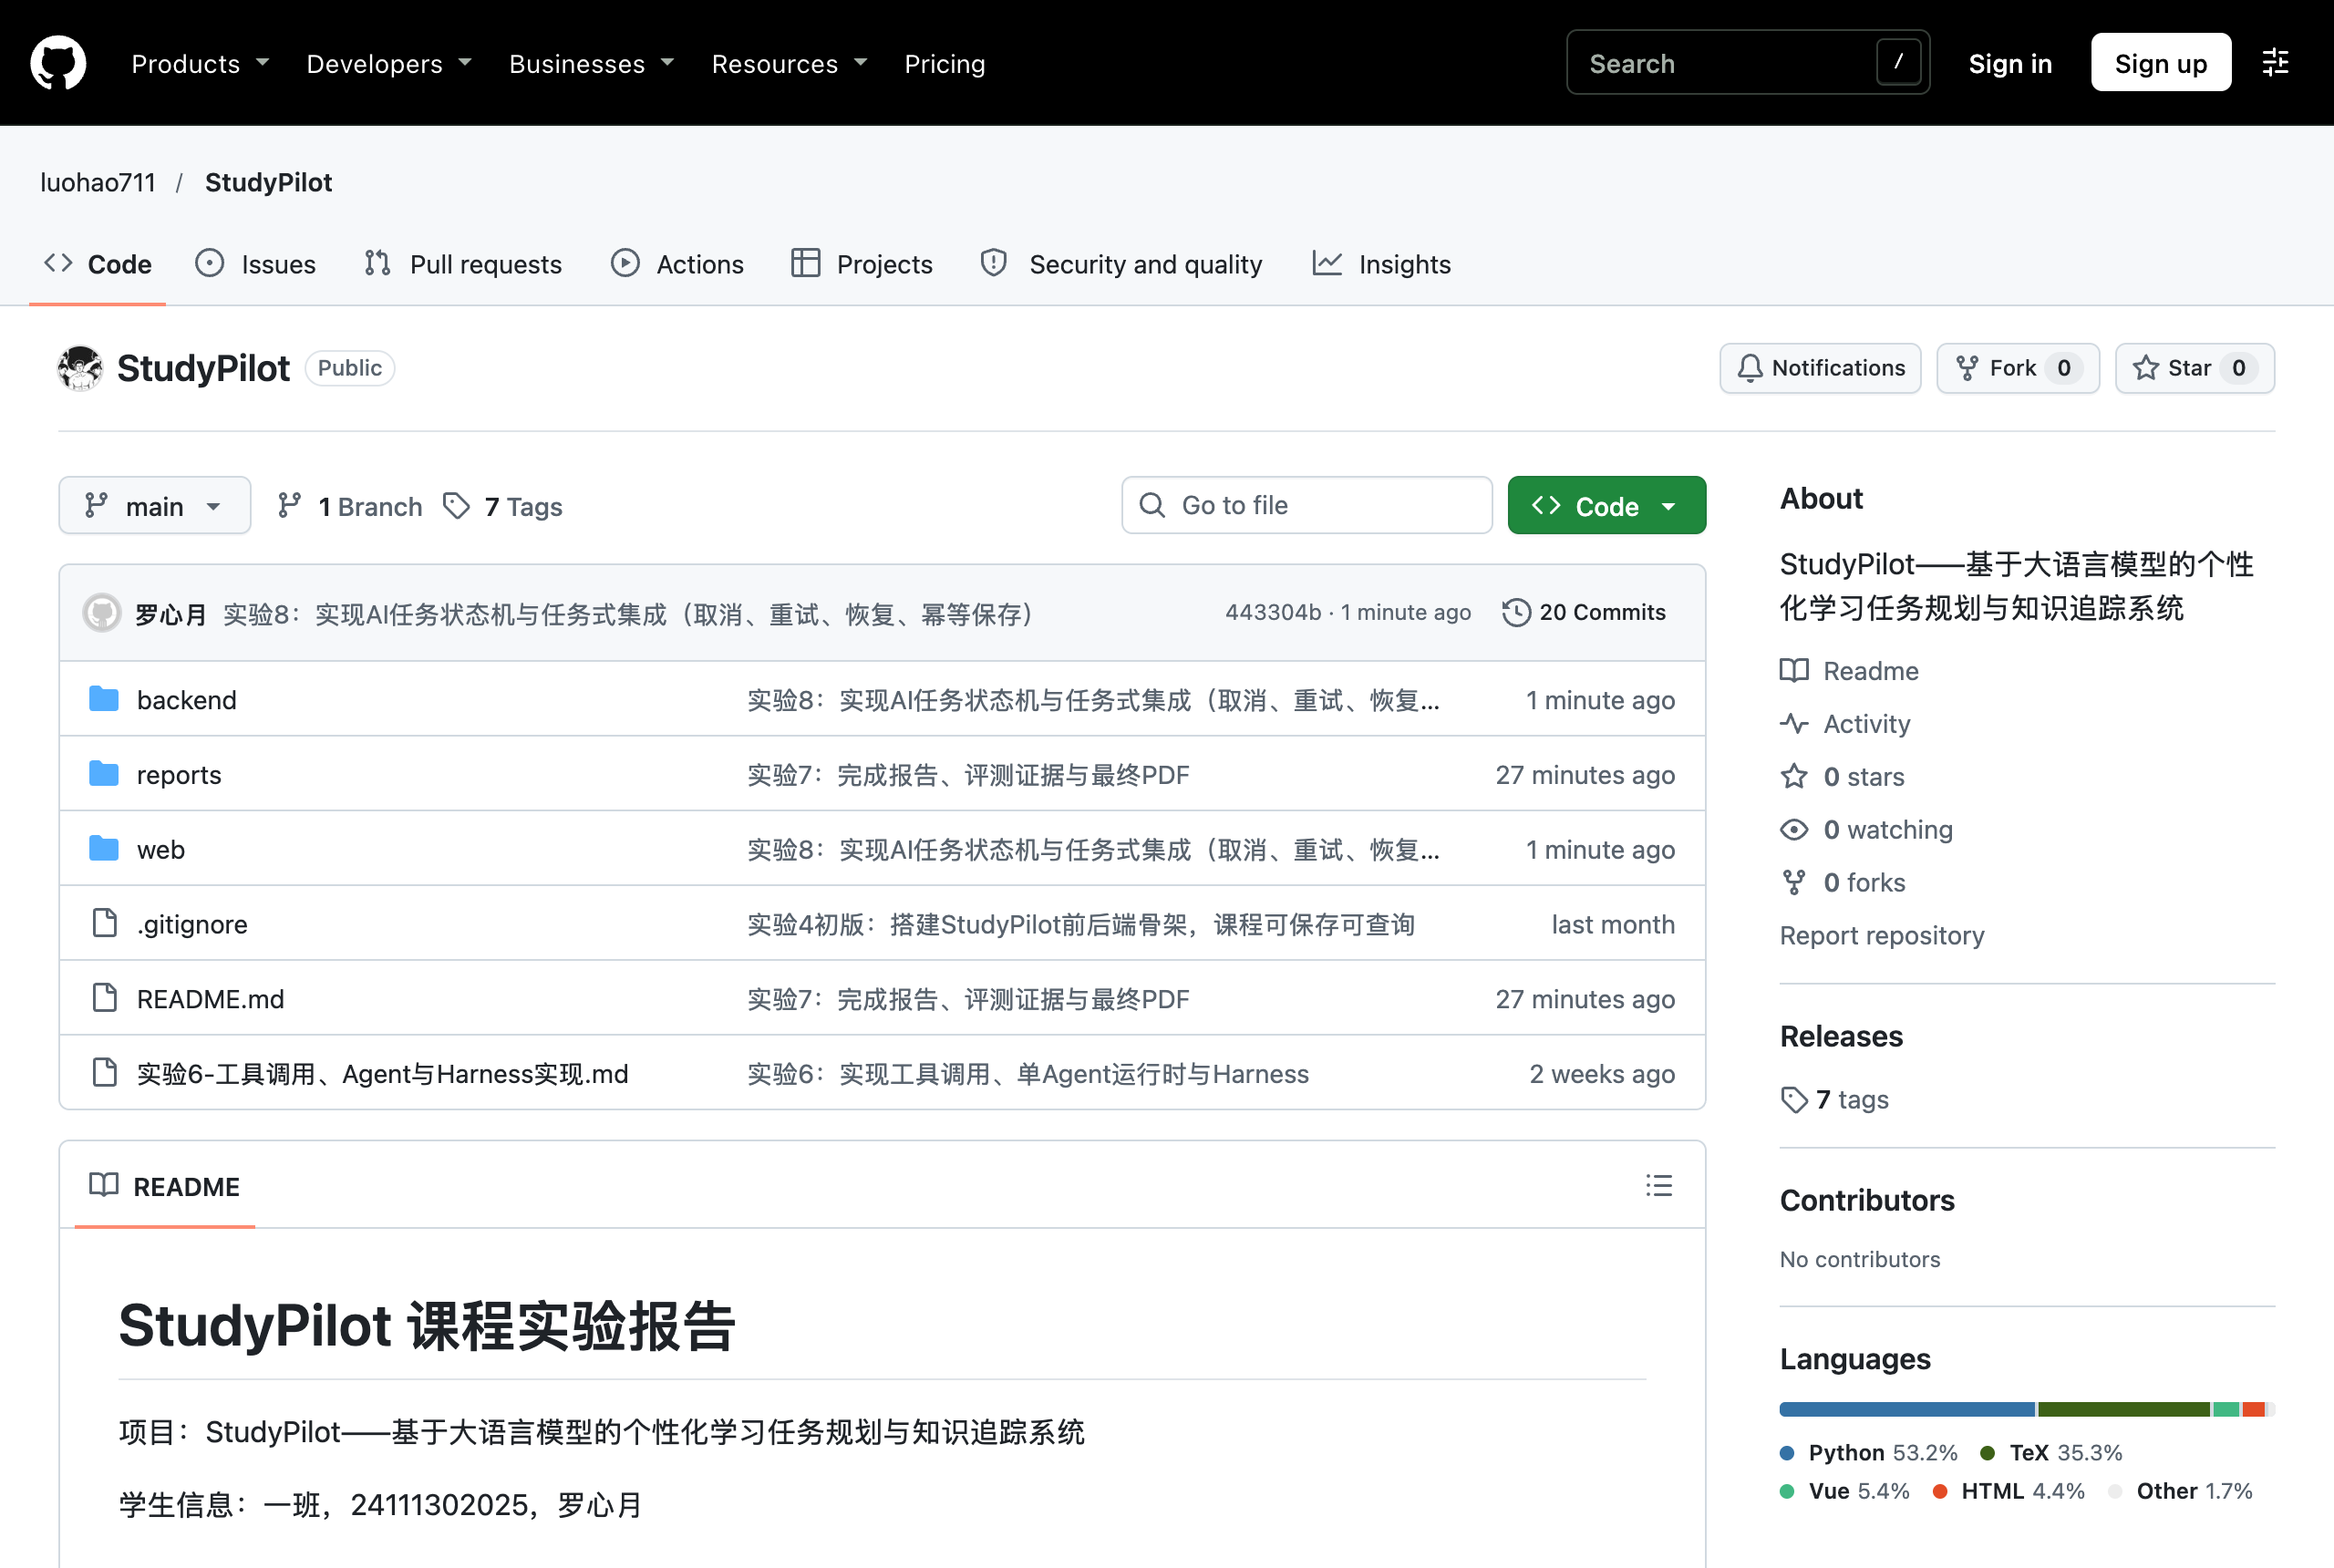
\includegraphics[width=0.95\textwidth]{e8-github.png}
\caption{GitHub 仓库页面：最新提交 443304b，仓库包含 backend、web、reports 三部分}
\label{fig:github}
\end{figure}

\section*{4. 实验小结}

本次实验把实验7的AI学习计划能力接入了实验4的基础软件，重点不在重新做模型，而在处理“模型调用放进真实软件”之后的问题。集成边界选在页面入口和生成器之间：生成器、Prompt、validator、修复和降级保持不变，外面增加一个可查询、可取消、可重试、可恢复的AI任务层。统一后的任务有编号、状态、输入快照、结果、错误和时间，页面通过轮询拿状态，等待时显示“排队中/处理中”和已等待秒数，不编造百分比；成功后用户可以编辑、重新生成、放弃或改用规则计划，保存只接受成功任务并按任务编号幂等；取消只停止等待，迟到结果在写库前被丢弃；刷新和服务重启都有恢复或中断提示。

端到端验证覆盖了正常、错误输入、等待、取消、失败、重复提交、刷新恢复、交错任务和数据保存等14个用例，页面6个场景全部通过，自动化测试从63个增加到83个且全部通过；开发中实际发现并修复了并发重复提交返回500、降级结果误标为模型生成、切换课程不刷新、处理中查看历史丢失轮询四个缺陷。试用中一名同学两轮完成三条任务，按反馈修改了状态提示、降级文案和历史任务交互，第二轮在没有提示的情况下完成，说明核心流程可用。

对比v0.6，v0.7没有让模型更快（总生成时间接近），但把平均7.1秒的同步等待变成平均5.7毫秒的提交响应和可离开的等待，增加了任务状态、取消、恢复、幂等保存和失败重试。当前局限是：单用户本地应用，没有账号和权限控制；单进程线程池加SQLite，多进程部署需要改成数据库级任务锁或消息队列；任务记录只保留7天；保存会覆盖同一课程的旧计划，没有历史版本；试用只有1人、版本对比只有3次，结论以可复核的流程和状态为主。下一步先补多用户归属与权限、任务历史保留和日志轮转，再扩大试用与对比样本，最后考虑把“完成任务后的重排”接到同一任务框架里。

\end{document}
